%%%%%%%%%%%%%%%%%%%%%%%%%%%%%%%%%%%%%%%%%%%%%%%%%%%%%%%%%%%%%%%%%%%%%%
% Lớp 12 | Ứng dụng đạo hàm để khảo sát hàm số | Sự đồng biến và nghịch biến của hàm số
% Dạng 2D1?1-5: Toán thực tế ứng dụng sự đồng biến nghịch biến
% Số câu: 18  (sinh tự động bởi tach_cau.py; từ nay thầy sửa trực tiếp file này)
%%%%%%%%%%%%%%%%%%%%%%%%%%%%%%%%%%%%%%%%%%%%%%%%%%%%%%%%%%%%%%%%%%%%%%

%%%%%%%%%%%%%%%% TRẮC NGHIỆM 4 PHƯƠNG ÁN %%%%%%%%%%%%%%%%

% nguồn: Phan1_Lop_12_Dai_so_Chuong_1
\begin{ex}%[2D1H1-5]%[ma:e1d74550]
	Sự ảnh hưởng khi sử dụng một loại độc tố với vi khuẩn $X$ được một nhà sinh học mô tả bởi hàm số $P(t)=\dfrac{t+1}{t^2+t+4}$, trong đó $P(t)$ là  số lượng vi khuẩn sau $t$ giờ sử dụng độc tố. Vào thời điểm nào thì số lượng vi khuẩn $X$ bắt đầu giảm?
	 \choice
		 {Ngay từ lúc bắt đầu sử dụng độc tố}
		{Sau $0{,}5$  giờ}
		 {Sau $2$ giờ}
		{\True  Sau $1$ giờ}
	 \loigiai{
		Ta có $P'(t)=\dfrac{-t^2-2t+3}{\left(t^2+t+4\right)^2}=\dfrac{(t-1)(-t-3)}{\left(t^2+t+4\right)^2}  \quad (t>0)$.\\
		$\Rightarrow  P'(t)=0 \Leftrightarrow \hoac{&t=-3 \quad \text{ (loại)}\\&t=1 \quad \text{ (nhận)}.}$\\
		Bảng biến thiên 
		\begin{center}
			
\begin{tikzpicture}[scale=1,font=\footnotesize,line join=round,line cap=round,>=stealth]
				 \tkzTabInit[nocadre=false,lgt=1.5,espcl=2,deltacl=0.5]
					{$t$/.7,$P'(t)$/.7,$P (t)$/2} 
					 {$0$,$1$,$+\infty$}
				 \tkzTabLine{,+,$0$,-,}
				\tkzTabVar{-/$\dfrac{1}{4}$,+/$\dfrac{1}{3}$,-/$0$} 
			\end{tikzpicture}
		\end{center}
		Ta thấy hàm số đạt cực đại tại $t=1$ và $P'(t)<0, \forall t \in(1;+\infty)$ nên sau $1$ giờ  thì vi khuẩn bắt đầu giảm.
	} 
\end{ex}


%%%%%%%%%%%%%%%% ĐÚNG/SAI %%%%%%%%%%%%%%%%

% nguồn: Phan1_Lop_12_Dai_so_Chuong_1

%%%%%%%%%%%%%%%% TRẢ LỜI NGẮN %%%%%%%%%%%%%%%%

% nguồn: Phan2_Lop_12_Dai_so_Chuong_1
% nguồn: Phan2_Lop_12_Dai_so_Chuong_1
\begin{bt}%[2D1H1-5]%[ma:44c62d8b]
	Từ  năm 2004 đến năm 2019 doanh thu $R(t)$ (tính bằng triệu đô la) của McDonald's có thể được mô hình hóa bởi
	\begin{align*}
		R(t)=-130{,}769  t^3+2296{,}47 t^2-11493,5 t+35493,~(4 \leq t \leq 19),
	\end{align*}
	trong đó $t$ là đại diện cho năm, với $t=4$ tương ứng với năm 2004. Biết rằng $R'(t)$ là hàm tốc độ doanh thu theo thời gian. Tốc độ thay đổi  doanh thu của McDonald's lớn nhất vào năm nào? (Kết quả làm tròn đến hàng đơn vị, tính theo triệu đô la mỗi năm).
	\shortans{2006} 
	 \loigiai{
		Ta có hàm tốc độ doanh thu là $R'(t)=-392{,}307 t^2+4592{,}94  t-11493{,}5$.\\
		Cho $R''(t)=-784{,}614 t+4592{,}94=0 \Leftrightarrow  t \approx 6 ~\text {(nhận).}$\\
		Ta  có bảng biến thiên của hàm số
		\begin{center}
			
\begin{tikzpicture}[line join=round,line cap=round,>=stealth]
				\tkzTabInit[nocadre,lgt=1,espcl=3,deltacl=0.5] 
					 {$t$/.7,$R''$/.7,$R$/2}
					 {$4$,$6$,$19$}
				\tkzTabLine{,+,$0$,-,} 
				\tkzTabVar{-/$601$,+/$1941$,-/$-65851$} 
			\end{tikzpicture}
		\end{center}
		 Dựa bào bảng biến thiên ta thấy rằng tốc độ thay đổi doanh thu của McDonald’s lớn nhất vào năm 2006 (tương ứng với $t=6$).
	 }
\end{bt}

% nguồn: Phan2_Lop_12_Dai_so_Chuong_1
\begin{bt}%[2D1H1-5]%[ma:975373b3]
	Giả sử sự lây lan của một loại virus ở một địa phương có thể được mô hình hoá bằng hàm số $N(t)=-t^3+12t^2$, $0 \le t \le 12$, trong đó $N$ là số người bị nhiễm bệnh (đơn vị là trăm người) và $t$ là thời gian (tuần).  Gọi $(a;b)$ là khoảng thời gian lâu nhất mà số người bị nhiễm bệnh tăng lên. Tính giá trị $P=2a^2-b^2$.
	 \shortans{-64}
	\loigiai{Để xác định khoảng thời gian số người  bị nhiễm bệnh tăng lên, ta xét các khoảng đồng biến, nghịch biến của hàm số $N(t)$.\\
		 Xét
		$N'(t)=0 \Leftrightarrow-3t^2+24t=0 \Leftrightarrow-3t(t-8)=0  \Leftrightarrow \hoac{&t=0\\&t=8}$.\\
		Bảng biến  thiên
		\begin{center}
			
\begin{tikzpicture}
				 \tkzTabInit[espcl=2.5,lgt=1.5]
					{$t$/0.7,$N'(t)$/0.7,$N (t)$/2.1} 
					 {$0$,$8$,$12$}
				 \tkzTabLine{0,+,0,-}
				 \tkzTabVar{-/$0$,+/$256$,-/$0$}
			\end{tikzpicture}
		\end{center}
		Số người bị nhiễm bệnh tăng lên khi $N'(t) > 0$,  tức là trên khoảng thời gian $(0;8)$.\\
		Đây là khoảng thời  gian lâu nhất mà số người bị nhiễm bệnh tăng lên.\\
		Do  đó $a=0$ và $b=8$.\\
	Tính giá trị $P=2a^2-b^2=2 \cdot  (0)^2-(8)^2=0-64=-64$.}
\end{bt}

% nguồn: Phan2_Lop_12_Dai_so_Chuong_1
\begin{bt}%[2D1H1-5]%[ma:5f171e86]
	Một cửa hàng quần áo đã thống kê số lượng quần áo bán ra trong ngày thứ $x$ ($1 \le x \le 30$) của một tháng xác định tuân theo quy luật được mô hình hoá bởi hàm số $f(x)=3x^2- 54x+256$. Hỏi trong tháng đó, có bao nhiêu ngày có số lượng quần áo bán ra nhiều hơn ngày  hôm trước?
	\shortans{21} 
	 \loigiai{Ta có $f'(x)=6x-54$.\\
		$f'(x)=0 \Leftrightarrow 6x-54=0 \Leftrightarrow  x=9$.\\
		Bảng biến thiên 
		\begin{center}
			
\begin{tikzpicture}
				\tkzTabInit[espcl=2.5,lgt=1.5] 
					 {$x$/0.7,$y'$/0.7,$y$/2.1}
					{$-\infty$,$9$,$+\infty$} 
				 \tkzTabLine{,-,0,+}
				\tkzTabVar{+/$+\infty$,-/$13$,+/$+\infty$} 
			\end{tikzpicture}
		\end{center}
		Vậy, các  ngày trong tháng có số lượng quần áo bán ra nhiều hơn ngày hôm trước là khi $f'(x) > 0$, tức là $x > 9$.\\
		Vì $x$ là số ngày, $x$ bắt đầu từ $1$, nên các ngày có số lượng quần áo  bán ra nhiều hơn ngày hôm trước là từ ngày $x=10$ đến ngày $x=30$.\\
	Khi đó có $30-10+1=21$ ngày thoả mãn yêu cầu  bài toán.}
\end{bt}

% nguồn: Phan2_Lop_12_Dai_so_Chuong_1
\begin{bt}%[2D1H1-5]%[ma:9f6499f5]
	Xét một chất điểm chuyển động trên một trục số nằm ngang, chiều dương từ trái sang phải. Giả sử vị trí $s(t)$  (mét) của chất điểm trên trục số đã chọn tại thời điểm $t$ (giây) được cho bởi công thức $s(t)=t^3-9t^2+15t$, $t \ge 0$. Hỏi chất điểm chuyển động sang trái trong khoảng thời gian bao nhiêu giây?
	\shortans{4} 
	\loigiai{Vận tốc của chất điểm là $v(t)=s'(t)=\left(t^3 -  9t^2+15t\right)'=3t^2-18t+15$.\\
		Chất  điểm chuyển động sang trái khi $v(t) < 0$.\\
		\begin{eqnarray*}
			v(t) < 0 &\Leftrightarrow& 3t^2-18t+15 <  0\\
			&\Leftrightarrow& t^2-6t+5  < 0\\
			 &\Leftrightarrow& (t-1)(t-5) < 0\\
			&\Leftrightarrow&  1 < t < 5.
		\end{eqnarray*}
		Chất điểm chuyển động theo chiều âm (từ phải sang trái) khi $v(t) < 0$, tức là $1 < t  < 5$.\\
	Vậy, trong khoảng thời gian $5-1=4$ (giây) thì chất điểm chuyển động  sang trái.}
\end{bt}

% nguồn: Phan2_Lop_12_Dai_so_Chuong_1
\begin{bt}%[2D1V1-5]%[ma:788eec77]
	Anh Nam có một cái ao với diện tích $50 \, \text{ cm}^2$ để nuôi cá điều hồng. Vu vơ qua, anh nuôi cá mật độ $40 \, \text{ con}/\text{ m}^2$ và thu được $3$ tấn cá thành phẩm. Theo kinh  nghiệm nuôi cá của mình anh thấy cứ thả giảm đi $8 \, \text{ con}/\text{ m}^2$ thì mỗi con cá thành phẩm thu được tăng thêm $0{,}5$ kg. Để tổng năng suất cao nhất thì vu tới anh Nam nên mua bao~nhiêu cá giống để thả? (giả sử không có hao hụt trong quá trình nuôi)
	\shortans{1600} 
	\loigiai{ 
		Số kilogram thành phẩm của  mỗi con cá lần nuôi đầu là $\dfrac{3\,000}{40{,}50} = 1{,}5 \, \text{ kg}$.\\
		Gọi $x$ là lượng cá sẽ giảm trên  mỗi $m^2$.\\
		Khi đó  khối lượng trung bình của mỗi con cá khi đó là $1{,}5 + \dfrac{x}{8} ,0{,}5 \, \text{ kg}$.\\
		Tổng lượng cá lúc đó là $(40 -  x)\cdot50$.\\
		Năng suất khi  đó là $f(x) = (40 - x)\cdot 50 \left(1{,}5 + \dfrac{0{,}5 x}{8}\right) = -3{,}125x^2 + 50x + 3\,000$.\\
		Năng suất lớn nhất đạt được tại $x = \dfrac{-b}{2a} = \dfrac{-50}{2(-3{,}125)} = 8$.\\ 
		Như  vậy can giảm $8 \, \text{ con}/\text{ m}^2$ để đạt năng suất lớn nhất.\\
		Tổng lượng cá cần thả để đạt năng suất tốt nhất là $(40 - 8)\cdot50 = 1\,600 \, \text{ con}$. 
	} 
\end{bt}

% nguồn: Phan2_Lop_12_Dai_so_Chuong_1
\begin{bt}%[2D1V1-5]%[ma:a77e40fe]
	Trong một thí nghiệm y học, người ta cấy $100000$ con vi khuẩn vào môi trường dinh dưỡng. Bằng thực nghiệm người  ta xác định được số lượng vi khuẩn N thay đổi theo thời gian bằng công thức $N(t)=80t^{3}-3600t^{2}+48000t+100000$ (thời gian $t$ tính bằng giây $0 \leq t \leq 45$). Gọi $(a;b)$ là khoảng thời gian dài nhất để vi khuẩn tăng. Hiệu $a-b$ bằng bao nhiêu?
	\shortans{-25} 
	 \loigiai{
		Ta có $N(t)=80t^{3}-3600t^{2}+48000t+100000 \Rightarrow N'(t)=240 t^{2}-7200t+48000$.\\ 
		$N'(t)=240t^{2}-7200t+48000=0  \Leftrightarrow\hoac{&t=10\\&t=20.}$\\
		Bảng biến  thiên
		\begin{center}
			
\begin{tikzpicture}
				\tkzTab 
					 [lgt=2,espcl=3]
					{$x$/1,$f’(x)$/1,$f (x)$/2.5} 
					{$0$,$10$,$20$,$45$} 
					 {,+,0,-,0,+,}
					 {-/,+/,-/,+/}
			\end{tikzpicture}
		\end{center}
		Vậy vi khuẩn tăng trong khoảng thời  gian lâu nhất là $(20;45) \Rightarrow\heva{&a=20\\&b=45} \Rightarrow a-b=-25$.
	 }
\end{bt}

% nguồn: Phan2_Lop_12_Dai_so_Chuong_1
\begin{bt}%[2D1V1-5]%[ma:eb1e61b5]
	Vận tốc dòng xe trên một đoạn đường quốc lộ $123$ từ $6$ giờ sáng đến $10$ giờ sáng trong ngày thường được xấp xỉ bởi $f(t)=20t-40\sqrt{t}+52$, $0 \le t  \le 4$, trong đó $f(t)$ đo bằng km/giờ và $t$ đo bằng giờ, với $t=0$ ứng với 6 giờ sáng. Qua đó người ta tìm được vào buổi sáng, tốc độ dòng xe giảm từ $a$ giờ đến $b$ giờ. Tìm $b$.
	\shortans{7} 
	\loigiai{Để tìm khoảng thời gian tốc độ dòng xe  giảm, ta xét đạo hàm của hàm số $f(t)$.\\
		Đạo hàm: $f'(t)=\left(20t-40\sqrt{t}+52\right)'=20-40  \cdot \dfrac{1}{2\sqrt{t}}=20-\dfrac{20}{\sqrt{t}}$.\\
		Với $f'(t)=0\Leftrightarrow 20-\dfrac{20}{\sqrt{t}}=0\Rightarrow=1$.\\ 
		 Xét dấu $f'(t)$
		\begin{itemize}
			\item Với $0 < t < 1$: $20-\dfrac{20}{\sqrt{t}} < 0 \Rightarrow f'(t) < 0$. Do đó $f(t)$ nghịch biến trên $(0,1)$. 
			 \item Với $1 < t \le 4$: $20-\dfrac{20}{\sqrt{t}} > 0 \Rightarrow f'(t) > 0$. Do đó $f(t)$ đồng biến trên $(1,4)$.
		\end{itemize}
		Tốc độ dòng xe giảm  khi $f'(t) < 0$, tức là trong khoảng thời gian $0 < t < 1$.\\
		Khi đó $t=0$ ứng với 6 giờ sáng và  $t=1$ ứng với $6+1=7$ giờ sáng.\\
	Vậy giá trị của $b$ là 7.} 
\end{bt}

% nguồn: Phan2_Lop_12_Dai_so_Chuong_1
\begin{bt}%[2D1V1-5]%[ma:0d7aea45]
	Trong một thí nghiệm y học, người ta cấy $100\,000$ con vi khuẩn vào môi trường dinh dưỡng. Bằng thực nghiệm người ta xác  định được số lượng vi khuẩn N thay đổi theo thời gian bằng công thức
	\begin{align*}
		N(t)=80  t^3-3\,600 t^2+48\,000 t+100\,000,
	\end{align*}
	(thời gian $t$ tính  bằng giây $0 \leq t \leq 45$). Gọi $(a; b)$ là khoảng thời gian tốc độ tăng trưởng của vi khuẩn giảm. Hiệu $b-a$ bằng bao~nhiêu?
	\shortans{25} 
	 \loigiai{
		Ta có $N(t)=80 t^3-3\,600 t^2+48\,000 t+100\,000 \Rightarrow  N'(t)=240 t^2-7\,200 t+48\,000$.\\
		Ta có $N'(t)=240  t^2-7\,200 t+48\,000=0 \Leftrightarrow \hoac{&t=10 \\& t=20.}$.\\
		Bảng biến thiên 
		\begin{center}
			
\begin{tikzpicture}[line join=round,line cap=round,>=stealth]
				 \tkzTabInit[nocadre,lgt=1.5,espcl=2,deltacl=0.5]
					{$x$/.7,$N'(t)$/.7,$N  (t)$/2}
					 {$0$,$10$,$20$,$45$}
				\tkzTabLine{,+,$0$,-,$0$,+,} 
				\tkzTabVar{-/$ $,+/$ $,-/$ $,+/$ $} 
			\end{tikzpicture}
		\end{center}
		Vậy  tốc độ tăng trưởng của vi khuẩn giảm trong khoảng thời gian $(20; 45)$.\\
		Vậy $a=20$, $b=45  \Rightarrow b-a=25$.
	 }
\end{bt}

% nguồn: Phan2_Lop_12_Dai_so_Chuong_1
\begin{bt}%[2D1V1-5]%[ma:b8e73a66]
	Ở một giải đua ô tô địa hình, một vận động cần hoàn thành chặng đường từ $A$ đến $B$ gồm $3$ đoạn: đường bằng, leo dốc và xuống dốc như hình vẽ bên dưới. Trên đoạn đường bằng $AC$ dài $10$km, xe chạy với vận tốc $100$km/h. Xe leo dốc $CD$ với vận tốc là $10$ km/h và xe xuống dốc $DB$ với vận tốc là $50$ km/h. Biết rằng: $BC=20$ km, $\widehat{DCB}=45^\circ$ và $\widehat{DBC}=30^\circ$. Hỏi vận động viên mất bao nhiêu giờ để hoàn thành chặng đường  từ $A$ đến $B$? (các kết quả làm tròn đến hàng phần trăm).
	\begin{center}
		\begin{tikzpicture}[scale=1,line cap=round,line join=round,font=\footnotesize,>=stealth]
			 \def\a{2}
			\path (0,0) coordinate  (A)
				 (0:\a) coordinate (C)++(45:.1) coordinate (c)
				(0:3*\a) coordinate (B)++(150:.1)  coordinate (b)
				(intersection of C--c  and B--b) coordinate (D);
			 \draw (A)--(C)--(D)--(B);
			 \foreach \a/\b in {A/-90,C/-90,D/40,B/-30}{
				\fill  (\a) circle (.7pt)
				 ($(\a)+(\b:2mm)$) node[scale=.8]{$\a$};
			} 
		\end{tikzpicture}
	\end{center}
	 \shortans{1,43}
	 \loigiai{
		Thời gian xe chạy trên đoạn đường bằng là $t_1=\dfrac{10}{100}=\dfrac{1}{10}$  (h).\\
		\begin{center}
			\begin{tikzpicture}[scale=1,line cap=round,line join=round,font=\footnotesize,>=stealth]
				\def\a{2} 
				\path (0,0)  coordinate (A)
					(0:\a) coordinate  (C)++(45:.1) coordinate (c)
					(0:3*\a)  coordinate (B)++(150:.1) coordinate (b)
					(intersection of C--c and B--b) coordinate  (D);
				\draw pic[draw,angle radius=2mm,angle eccentricity=2.5,"\tiny $45^\circ$"]{angle=  B--C--D};
				\draw pic[draw,double,angle radius=3mm,angle eccentricity=2,"\tiny  $30^\circ$"]{angle= D--B--C};
				\draw (A)--(C)--(D)--(B)--(C); 
				\foreach  \a/\b in {A/-90,C/-90,D/40,B/-30}{
					\fill (\a) circle (.7pt) 
					 ($(\a)+(\b:2mm)$) node[scale=.8]{$\a$};
				 }
			\end{tikzpicture}
		\end{center}
		 Ta có $\widehat{BDC}=180^\circ -\left(\widehat{DCB}+\widehat{DBC}\right)=105^\circ$.\\
		Áp dụng định lý sintrong  $\triangle BCD$, ta có
		$\dfrac{BC}{\sin \widehat{BDC}}=\dfrac{CD}{\sin \widehat{DBC}}=\dfrac{BD}{\sin \widehat{DCB}}$.\\ 
		Suy ra $CD=\dfrac{20\cdot \sin  30^\circ}{\sin 105^\circ}=10\sqrt{6}-10\sqrt{2}$ (km) và $BD=\dfrac{20\cdot \sin 45^\circ}{\sin 105^\circ}=20\sqrt{3}-20$ (km).\\
		 Thời gian xe chạy trên đoạn đường leo dốc là $t_2=\dfrac{10\sqrt{6}-10\sqrt{2}}{10}=\sqrt{6}-\sqrt{2}$ (h).\\
		Thời  gian xe chạy trên đoạn đường xuống dốc là $t_3=\dfrac{20\sqrt{3}-20}{50}=\dfrac{2\sqrt{3}-2}{5}$ (h).\\
		Tổng thời gian vận động viên hoàn  thành chặng đường từ $A$ đến $B$ là
		 \[t_1+t_2+t_3=\dfrac{1}{10}+\sqrt{6}-\sqrt{2}+\dfrac{2\sqrt{3}-2}{5}\approx 1{,}43 \mathrm{~(h)}.\]
		Vậy vận động viên mất $1{,}43$ giờ để hoàn thành chặng đường từ $A$  đến $B$.
	 }
\end{bt}

% nguồn: Phan2_Lop_12_Dai_so_Chuong_1
\begin{bt}%[2D1V1-5]%[ma:9a827204]
	Một công ty sản xuất sản phẩm và doanh thu (đơn vị: triệu đồng) từ việc bán sản phẩm được mô tả bởi hàm số $R(x)=-2x^3+9x^2+12x+100$. Trong đó, $x$ là số lượng sản phẩm được bán ra (tính bằng ngàn sản phẩm). Hỏi số lượng sản phẩm tối thiểu phải bán ra để doanh thu bắt đầu tăng là bao nhiêu sản phẩm? (Kết quả làm tròn đến  hàng đơn vị).
	 \shortans{3,56}
	\loigiai{ 
		 Ta có $R(x)=-2x^3+9x^2+12x+100$.\\
		Tập xác định  $\mathscr{D}=(0,+\infty)$.\\
		$\Rightarrow R'(x)=-6x^2+18x+12=0  \\
		 \Rightarrow x=\dfrac{3-\sqrt{17}}{2}$ hoặc $x=\dfrac{3+\sqrt{17}}{2}\approx3{,}5616$.
		\begin{center}
			
\begin{tikzpicture}[line join=round,line cap=round,>=stealth,font=\footnotesize,scale=1]
				 \tkzTabInit
					 {$x$/1,$R'(x)$/1,$R (x)$/3}
					{$0$,$\dfrac{3+\sqrt{17}}{2}$,$+\infty$} 
				\tkzTabLine{,-,0,+,} 
				\tkzTabVar{+/$0$,-/$-14{,}16$,+/$+\infty$} 
			\end{tikzpicture}
		\end{center}
		Do vậy số lượng sản  phẩm tối thiểu phải bán ra để doanh thu bắt đầu tăng là
		\begin{center}
			$3,5616\cdot 1\,000=3\,561{,}6$  hay $3\,562$ sản phẩm.
		\end{center}
	} 
\end{bt}

% nguồn: Phan2_Lop_12_Dai_so_Chuong_1
% nguồn: Phan2_Lop_12_Dai_so_Chuong_1
\begin{bt}%[2D1V1-5]%[ma:5068cb23]
	Nồng độ thuốc trong máu của  một bệnh nhân sau khi tiêm $t$ giây là $P(t)\left(\dfrac{\text{ mg}}{\text{ ml}}\right)$. Với $P(t)$ cho bởi công thức
	\begin{align*}
		P(t)=\sqrt{0,09 t^2+0{,}018 t+0{,}05}-0{,}3  t.
	\end{align*}
	Nồng độ thuốc tồn dư, tức nồng độ  thuốc vẫn còn trong cơ thể bệnh nhân trong dài hạn khi tiêm là bao~nhiêu?
	 \shortans{0,03}
	\loigiai{ 
		Do đề bài cho nồng độ  thuốc trong cơ thể bệnh nhân trong dài hạn nên $t \to +\infty$.\\
		Ta có\allowdisplaybreaks 
		\begin{eqnarray*}
			 \lim\limits _{t \rightarrow+\infty} P(t)
			&=&\lim\limits  _{t \rightarrow+\infty}\left(\sqrt{0{,}09 t^2+0{,}018 t+0{,}05}-0{,}3 t\right)\\
			&=&\lim\limits _{t  \rightarrow+\infty} \dfrac{0{,}09 t^2+0{,}018 t+0{,}05-(0{,}3 t)^2}{\sqrt{0{,}09 t^2+0{,}018 t+0{,}05}+0{,}3 t} \\
			&=&\lim\limits _{t  \rightarrow+\infty} \dfrac{0{,}018 t+0{,}05}{\sqrt{0{,}09 t^2+0{,}018 t+0{,}05}+0{,}3 t}\\
			&=&\lim\limits _{t \rightarrow+\infty} \dfrac{t\left(0{,}018+\dfrac{0{,}05}{t}\right)}{t\left(\sqrt{0{,}09+\dfrac{0{,}018}{t}+\dfrac{0{,}05}{t^2}}+0{,}3\right)}\\ 
			&=&\lim\limits _{t \rightarrow+\infty} \dfrac{0{,}018+\dfrac{0{,}05}{t}}{\sqrt{0{,}09+\dfrac{0{,}018}{t}+\dfrac{0{,}05}{t^2}}+0{,}3}\\ 
			 &=&\dfrac{0{,}018}{\sqrt{0{,}09}+0{,}3}=0{,}03.
		\end{eqnarray*}
		Vậy nồng độ thuốc tồn dư trong cơ thể bệnh  nhân là $0{,}03~\left(\dfrac{\text{ mg}}{\text{ ml}}\right)$.
	 }
\end{bt}


%%%%%%%%%%%%%%%% TỰ LUẬN %%%%%%%%%%%%%%%%

% nguồn: Phan2_Lop_12_Dai_so_Chuong_1
\begin{bt}%[2D1H1-5]%[ma:d04327be]
	Giả sử một hạt chuyển động trên một trục thẳng đứng chiều dương hướng lên trên  sao cho toạ độ của hạt (đơn vị: mét) tại thời điểm $t$ (giây) là $y=t^3-12t+3, t \geq 0$. Tính quãng đường của hạt đi được trong $3$ giây đầu tiên.
	 \loigiai{
		Vận tốc của  hạt chuyển động là $v(t)=y'=3t^2-12$.\\
		Gia tốc của hạt chuyển động là $a(t)=v'(t)=6t$, suy ra  $a(2)=12$.\\
		 Hạt chuyển động đi xuống khi $v(t)\le 0\Leftrightarrow 0\le t\le 2$.\\
		Hạt chuyển động đi lên khi $v(t)\ge0 \Leftrightarrow t\ge 2$.\\ 
		Khi $0\le t\le 2$, hạt chuyển động đi xuống nên quãng đường đi được trong khoảng thời gian $0\le t \le 2$ là  $y(0)-y(2)=16$.\\
		Khi $2\le t\le 3$, hạt chuyển động đi lên nên quãng đường đi được là trong khoảng  thời gian $2\le t \le 3$ là $y(3)-y(2)=7$.\\
		 Do đó quãng đường đi được trong khoảng thời gian $0\le t \le 3$ là $23$ m.
	 }
\end{bt}

% nguồn: Phan2_Lop_12_Dai_so_Chuong_1
\begin{bt}%[2D1H1-5]%[ma:414b601d]
	Trong $8$ phút đầu kể từ khi xuất phát, độ cao $h$ (tính bằng mét) của khinh khí cầu vào thời điểm $t$ phút được cho bởi công thức $h(t) = 6t^3 - 81t^2+324t$. Trong các khoảng thời gian nào khinh khí cầu tăng dần độ  cao, giảm dần độ cao?
	 \loigiai{
		Xét hàm số $h(t) = 6t^3 - 81t^2+324t$ trên đoạn $[0;8]$.\\ 
		Ta có $h'(t)=18t^3 - 162t+324$, $h'(t)=0\Leftrightarrow 18t^3 -  162t+324 =0\Leftrightarrow \hoac{&t=3\\&t=6.}$\\
		Bảng biến  thiên
		\begin{center}
			
\begin{tikzpicture}[font=\footnotesize,>=stealth]
			\tikzset{double style/.append style={double distance=1.5pt}}
			\tkzTabInit[nocadre=false,lgt=1.2,espcl=2.5,deltacl=0.6] 
				{$xt$ /0.6,$h'(t)$  /0.6,$h (t)$ /2}
				{$0$,$3$,$6$,$8$} 
			\tkzTabLine{,+,z,-,z,+,} 
			\tkzTabVar{-/$0$,+/$405$,-/$324$,+/$480$} 
		\end{tikzpicture}
		\end{center}
		 Từ bảng biến thiên suy ra\\
		Hàm số $h(t)$ đồng biến trên các khoảng $(0; 3)$ và $(6; 8)$, nghịch biến trên khoảng  $(3;6)$.\\
		Do đó trong khoảng thời gian từ $0$ đến $3$ phút và từ $6$ đến $8$ phút  thì khinh khí cầu tăng dần độ cao. Trong khoảng thời gian từ $3$ đến $6$ phút thì khinh khí cầu giảm dần độ cao.
	 }
\end{bt}

% nguồn: Phan2_Lop_12_Dai_so_Chuong_1
\begin{bt}%[2D1V1-5]%[ma:1b003e54]
	Thể tích $V$ (đơn vị: centimét khối) của $1$ kilogam nước tại nhiệt độ  $T\,(0^{\circ} \mathrm{C} \leq T \leq 30^{\circ} \mathrm{C})$ được tính bởi công thức
	 $$
	V(T)=999{,}87-0{,}06426 T+0{,}0085043 T^2-0{,}0000679  T^3.
	$$ 
	Hỏi thể tích  $V(T)$, với $0^{\circ} \mathrm{C} \leq T \leq 30^{\circ} \mathrm{C}$, giảm trong khoảng nhiệt độ nào?
	 \loigiai{
		Xét hàm số $V(T)=999{,}87-0{,}06426 T+0{,}0085043 T^2-0{,}0000679 T^3$ với $T \in[0; 30]$.\\ 
		 Ta có $V'(T)=-0{,}0002037 T^2+0{,}0170086 T-0{,}06426$.\\
		Khi đó $V'(T)=0 \Leftrightarrow\hoac{&T=3{,}966514624=T_1  \\& T=79{,}53176716 \notin[0; 30].}$\\
		Bảng  biến thiên của hàm số $V(T)$ như sau.
		\begin{center}
			
\begin{tikzpicture}
				 \tkzTabInit[nocadre=true,lgt=1.3,espcl=4,deltacl=0.6]
					 {$T$/0.7,$V'(T)$/0.7,$V (T)$/2}
					 {$0$,$T_1$,$30$}
				\tkzTabLine{,-,$0$,+,} 
				\tkzTabVar{+/$V  (0)$,-/$V (T_1)$,+/$V (30)$}
			\end{tikzpicture}
		\end{center}
		Từ bảng biến thiên suy ra thể tích $V(T),\, 0^{\circ} \mathrm{C} \leq  T \leq 30^{\circ} \mathrm{C}$, giảm trong khoảng nhiệt độ $0^{\circ} \mathrm{C}$ đến nhiệt độ $3{,}966514624^{\circ} \mathrm{C}$.
	} 
\end{bt}

% nguồn: 2026-11-16_12_2D1_TL_Ham_so (nhập 16/11/2026)
\begin{bt}%[2D1V1-5]%[ma:1c9b312b]
% nguon: Archive/SP_SauLuoi_2024-2025/SP_HKI/2-TN-DS-TL-SGD-HUE-HKI-N24-25.tex #46
%[Lớp 12- Kiểm tra học kỳ I- SGD-HUẾ]%[Nguyễn Văn Sang]
    Một chất điểm đang chuyển động trên một đường thẳng và gặp một con dốc cao muốn vượt qua. Xem chân dốc là điểm $A$, khi chất điểm qua $A$ là thời điểm bắt đầu leo dốc với phương trình chuyển động là $s(t) = at - 2t^2$ cho đến khi lên đỉnh dốc ($a$ là tham số thực dương, $t \geq 0$ tính bằng giây và $s$ tính bằng mét). Biết dốc có độ dài bằng $50m$ và xe muốn leo dốc thành công thì phải tồn tại $t > 0$ sao cho $s(t) = 50$. Tính vận tốc ban đầu nhỏ nhất để xe leo dốc thành công.
    \loigiai{
        Ta có phương trình chuyển động của chất điểm $s(t) = at - 2t^2$.\\
        Để xe leo dốc thành công thì phải tồn tại $t > 0$ sao cho $s(t) = 50$, hay $at - 2t^2 = 50$ hay $2t^2 - at + 50 = 0$.\\
        Để phương trình trên có nghiệm $t > 0$ thì trước hết $\Delta \geq 0$, tức là $$(-a)^2 - 4.2.50 \geq 0 \Leftrightarrow a^2 \geq 400 \Leftrightarrow a \geq 20 \left(\text{ do } a>0\right).$$
       Gọi $t_1, t_2$ là hai nghiệm của phương trình $2t^2 - at + 50 = 0$. Theo định lý Viète, ta có
	   $$\heva{&t_1 + t_2 = \dfrac{a}{2}\\&t_1 t_2 = \dfrac{50}{2} = 25.}$$
       Để tồn tại nghiệm $t>0$, ta có $2$ trường hợp xảy ra
       \begin{itemize}
           \item  Cả $2$ nghiệm đều dương $\Leftrightarrow t_1 + t_2 > 0$ và $t_1t_2 >0$ (đã thoả mãn).
           \item Có $1$ nghiệm dương và 1 nghiệm âm. Lúc này ta có $t_1t_2<0$. Điều này mâu thuẫn với $t_1t_2=25>0$, vậy trường hợp này không xảy ra.
       \end{itemize}
        Vậy điều kiện để phương trình có nghiệm dương là  $\Delta \geq 0 \Leftrightarrow a\geq 20$.\\
        Vận tốc của chất điểm là $v(t) = s'(t) = a - 4t$. Vận tốc ban đầu ứng với $t=0$ là $v(0) = a$.\\
        Để xe leo dốc thành công thì phương trình $at - 2t^2 = 50$ phải có nghiệm dương, tức là $a \geq 20$.\\
        Vậy vận tốc ban đầu nhỏ nhất để xe leo dốc thành công là $20$ m/s.
    }
\end{bt}

% nguồn: 2026-11-16_12_2D1_TL_Ham_so (nhập 16/11/2026)
\begin{bt}%[2D1V1-5]%[ma:6fe13721]
% nguon: Archive/2024/0. [LVH] BG - 12 New - 4in1-20240625T224301Z-001/0. [LVH] BG - 12 New - 4in1/2. [LVH] TEX SGK 12 NEW-20240418T074833Z-001/2. [LVH] TEX SGK 12 NEW/[LVH] CD-12new/SGK-12-CD/data/12-SGK-CD-1-1.tex #1075

	Thể tích $V$ (đơn vị: centimét khối) của $1$ kg nước tại nhiệt độ $T\left(0^{\circ}\mathrm{C}\leq T \leq 30^{\circ}\mathrm{C}\right)$ được tính bởi công thức sau:
	$$V(T)=999{,}87-0{,}06426T+0{,}0085043T^2-0{,}0000679T^3.$$
	\centerline{
	(Nguồn: J. Srewart, Calculux, Sevenuh Ediriom, Brooks/Cole, CENGAGE Leaming 2012)}\\
	Hỏi thể tích $V(T), 0^{\circ}\mathrm{C}\leq T \leq 30^{\circ}\mathrm{C}$, giảm trong khoảng nhiệt độ nào?
	\loigiai{
	Xét hàm số  $V(T)=999{,}87-0{,}06426T+0{,}0085043T^2-0{,}0000679T^3$, với $T\in [0;30]$.\\
	Ta có $V'(T)=-0{,}0002037T^2+0{,}0170086T-0{,}06426$.\\
	$V'(T)=0\Leftrightarrow T=3{,}966514624=T_1$ hoặc $T=79{,}53176716\not\in [0;30]$.\\
	Bảng biến thiên của hàm số $V(T)$ như sau
	\begin{center}
	
\begin{tikzpicture}[font=\footnotesize,thick,>=stealth]
		\tikzset{double style/.append style={double distance=1.5pt}}
		\tkzTabInit[nocadre=false,lgt=1.2,espcl=2.5,deltacl=0.6,lw=.75pt,color,colorL=green!50,colorV=green!50]
		{$T$ /0.7, $V'(T)$ /0.8, $V(T)$ /2}
		{$0$,$T_1$,$30$}
		\tkzTabLine{ ,-,$0$,+, }
		\tkzTabVar{+/$V(0)$,-/$V(T_1)$,+/$V(30)$}
	\end{tikzpicture}
	\end{center}
	Từ bảng biến thiên suy ra, thể tích $V(T), 0^{\circ}\mathrm{C}\leq T \leq 30^{\circ}\mathrm{C}$, giảm trong khoảng nhiệt độ từ $0^\circ$C đến $3{,}966514624^\circ$C.
	}
\end{bt}

% nguồn: 2026-11-16_12_2D1_TL_Ham_so (nhập 16/11/2026)
% nguồn: 2026-11-16_12_2D1_TL_Ham_so (nhập 16/11/2026)
\begin{bt}%[2D1V1-5]%[ma:2ff37b0f]
% nguon: Archive/2024/0. [LVH] BG - 12 New - 4in1-20240625T224301Z-001/0. [LVH] BG - 12 New - 4in1/2. [LVH] TEX SGK 12 NEW-20240418T074833Z-001/2. [LVH] TEX SGK 12 NEW/[LVH] SGK-12-KNTT/data/SCD/12-SCD-KNTT-1-2.tex #1170

	Tại một nhà máy sản xuất linh kiện điện tử, các linh kiện được xếp vào từng hộp một cách độc lập, mỗi hộp $10$ linh kiện. Hộp được xếp loại $I$ nếu hộp đó có nhiều nhất một linh kiện không đạt tiêu chuẩn. Biết rằng xác suất để nhà máy sản xuất ra một linh kiện điện tử không đạt tiêu chuẩn là $0{,}01$. Hỏi tỉ lệ những hộp linh kiện điện tử loại $I$ là bao nhiêu?
	\loigiai{
		Gọi $X$ là số linh kiện không đạt tiêu chuẩn thì $X$ là một biến ngẫu nhiên có phân bố nhị thức với tham số $n=10$, $p=0{,}01$.\\
		Hộp được xếp loại $I$ nếu hộp đó có nhiều nhất một linh kiện không đạt tiêu chuẩn tức là $X\le 1$.\\
		Theo chú ý về phân bố nhị thức ta có:
		$$\mathrm{P}(X\le 1)=\mathrm{C}^0_{10}\cdot \left(0{,}01\right)^0\cdot \left(0{,}99\right)^{10}+\mathrm{C}^1_{10}\cdot \left(0{,}01\right)^1\cdot \left(0{,}99\right)^{9}\approx 0{,}996.$$
		Vậy tỉ lệ những hộp linh kiện điện tử loại $I$ là $99{,}6\%$.
	}
\end{bt}

% nguồn: 2026-11-16_12_2D1_TL_Ham_so (nhập 16/11/2026)
\begin{bt}%[2D1V1-5]%[ma:5f4642ba]
% nguon: Archive/2024/0. [LVH] BG - 12 New - 4in1-20240625T224301Z-001/0. [LVH] BG - 12 New - 4in1/2. [LVH] TEX SGK 12 NEW-20240418T074833Z-001/2. [LVH] TEX SGK 12 NEW/[LVH] SGK-12-KNTT/data/SCD/12-SCD-KNTT-1-2.tex #1171

	Một bài thi trắc nghiệm gồm $10$ câu hỏi, mỗi câu có $4$ phương án trả lời, trong đó chỉ có một phương án đúng. Mỗi câu trả lời đúng được $4$ điểm, mỗi câu trả lời sai trừ $1$ điểm. Một thí sinh làm bài bằng cách ở mỗi câu hỏi chọn ngẫu nhiên một phương án trả lời. Tính xác suất để thí sinh đó sau khi hoàn thành hết $10$ câu trong bài thi, có kết quả:
	\begin{enumerate}[a)]
		\item $15$ điểm;
		\item Bị điểm âm.
	\end{enumerate}
	\loigiai{
		Gọi $X$ là số câu trả lời đúng của thí sinh. $X$ là một biến ngẫu nhiên có phân bố nhị thức với tham số $n=10$, $p=\dfrac{1}{4}$.
		\begin{enumerate}[a)]
			\item Thí sinh đạt $15$ điểm thì có $5$ câu trả lời đúng và $5$ câu trả lời sai, tức là $X=5$. Khi đó, xác suất là:
			$$\mathrm{P}=\mathrm{C}^5_{10}\cdot \left(\dfrac{1}{4}\right)^5\cdot \left(\dfrac{3}{4}\right)^5\approx 0{,}058.$$
			\item Thí sinh bị điểm âm tức là thí sinh trả lời đúng nhiều nhất $1$ câu, tức là $X\le 1$.\\
			Theo chú ý về phân bố nhị thức ta có:
			$$\mathrm{P}(X\le 1)=\mathrm{C}^0_{10}\cdot \left(\dfrac{1}{4}\right)^0\cdot \left(\dfrac{3}{4}\right)^{10}+\mathrm{C}^1_{10}\cdot \left(\dfrac{1}{4}\right)^1\cdot \left(\dfrac{3}{4}\right)^{9}\approx 0{,}24.$$
		\end{enumerate}
	}
\end{bt}

% nguồn: 2026-11-16_12_2D1_TL_Ham_so (nhập 16/11/2026)
\begin{bt}%[2D1V1-5]%[ma:06f12ebe]
% nguon: Archive/2024/0. [LVH] BG - 12 New - 4in1-20240625T224301Z-001/0. [LVH] BG - 12 New - 4in1/2. [LVH] TEX SGK 12 NEW-20240418T074833Z-001/2. [LVH] TEX SGK 12 NEW/[LVH] SGK-12-KNTT/data/SCD/12-SCD-KNTT-1-2.tex #1172

	Trong một trò chơi, mỗi ván người chơi gieo đồng thời $3$ xúc xắc cân đối, đồng chất. Nếu có ít nhất $2$ xúc xắc xuất hiện mặt $6$ chấm thì người chơi giành chiến thắng ván chơi đó. Bác Hưng tham gia chơi $3$ ván. Tính xác suất để bác Hưng thẳng ít nhất $2$ ván.
	\loigiai{
		Xác suất để một con xúc xắc xuất hiện mặt $6$ chấm là $\dfrac{1}{6}$.\\
		Gọ $X$ là số con xúc xắc xuất hiện mặt $6$ chấm.\\
		Bác Hưng thắng cuộc $1$ ván khi $X\ge 2$.\\
		Xác suất để bác Hưng thắng cuộc một ván là
		$$\mathrm{P}(X\ge 2)=\mathrm{C}^2_3\cdot \left(\dfrac{1}{6}\right)^2\cdot \dfrac{3}{4}+\left(\dfrac{1}{6}\right)^3=\dfrac{2}{27}.$$
		Gọi $Y$ là số ván thắng của bác Hưng.\\
		Xác suất để bác Hưng thắng ít nhất $2$ ván là
		$$\mathrm{P}(Y\ge 2)=\mathrm{C}^2_3\cdot \left(\dfrac{2}{27}\right)^2\cdot \dfrac{25}{27}+\left(\dfrac{2}{27}\right)^3=\dfrac{308}{19683}.$$
	}
\end{bt}

% nguồn: 2026-11-16_12_2D1_TL_Ham_so (nhập 16/11/2026)
\begin{bt}%[2D1V1-5]%[ma:3a9f1c2b]
% nguon: Archive/2024/0. [LVH] BG - 12 New - 4in1-20240625T224301Z-001/0. [LVH] BG - 12 New - 4in1/2. [LVH] TEX SGK 12 NEW-20240418T074833Z-001/2. [LVH] TEX SGK 12 NEW/[LVH] SGK-12-KNTT/data/SCD/12-SCD-KNTT-1-2.tex #1173

	Màu hạt của đậu Hà Lan có hai kiểu hình: màu vàng và màu xanh. Có hai gene ứng với hai kiểu hình này là allele trội $A$ và allele lặn $a$. Khi cho lai hai cây đậu Hà Lan, cây con lấy ngẫu nhiên một gene từ cây bố và một gene từ cây mẹ để hình thành một cặp gene.\\
	Bốn bạn An, Bình, Sơn và Dương, mỗi bạn độc lập với nhau, thực hiện phép thử là lai hai cây đậu Hà Lan, trong đó cây bố có kiểu gene là $Aa$, cây mẹ có kiểu gene là $Aa$.\\
	Gọi $X$ là số cây con có hạt màu vàng trong số $4$ cây con.
	\begin{enumerate}[a)]
		\item Lập bảng phân bố xác suất của $X$.
		\item Hỏi trung bình có bao nhiêu cây con có hạt màu xanh?
	\end{enumerate}
	
	\loigiai{
		Ta vẽ sơ đồ hình cây để mô tả các kết quả có thể của kiểu gene ứng với màu hạt của cây con.
		\begin{center}
			\begin{tikzpicture}
				\def\gocm{20}
				\def\gocn{10}
				\def\r{4}
				\tikzset{s/.style={outer sep=0.5 mm,draw=magenta,rectangle,minimum width=2.75cm,text width=2.75cm,align=center,rounded corners=1mm,minimum height=1cm}}
				\path(0,0)node(O){}++(\gocm:\r)node[s](A1){A}++(\gocn:\r)node[s](A2){A};
				\path(A1)++({-\gocn}:\r)node[s](a2){a};
				\path(O)++(-\gocm:\r)node[s](B1){a}++(\gocn:\r)node[s](B2){A};
				\path(B1)++({-\gocn}:\r)node[s](b2){a};
				\foreach \x/\y in {
					O/A1,A1/A2,O/B1,B1/B2,A1/a2,B1/b2}
				\draw[-stealth](\x.east)--(\y.west);
				\path(O)--(A1.west)node[pos=0.5,above,sloped]{}(O)--(B1.west)node[pos=0.5,below,sloped]{}(B1.east)--(B2.west)node[pos=0.5,above,sloped]{}(A1.east)--(A2.west)node[pos=0.5,above,sloped]{}
				(A1.east)--(a2.west)node[pos=0.5,below,sloped]{}
				(B1.east)--(b2.west)node[pos=0.5,below,sloped]{};
				%%Node dòng trên
				\path(A2)++(0,1)node{\textbf{Cây mẹ}}++(180:4)node{\textbf{Cây bố}};
				\node[left] at (O) {\textbf{GỐC}};
			\end{tikzpicture}
		\end{center}
		\begin{enumerate}[a)]
			\item $X$ là số cây con có hạt màu vàng trong số $4$ cây con. $X$ là một biến ngẫu nhiên có phân bố nhị thức với $n=4$, $p=\dfrac{3}{4}$. Giá trị của $X$ thuộc tập $\{0; 1; 2; 3; 4\}$. Ta có
			\begin{itemize}
				\item $\mathrm{P}(X=0)=\left(\dfrac{1}{4}\right)^4=\dfrac{1}{256}$;
				\item $\mathrm{P}(X=1)=\mathrm{C}^1_4\cdot \dfrac{3}{4}\cdot \left(\dfrac{1}{4}\right)^3=\dfrac{12}{256}$;
				\item $\mathrm{P}(X=2)=\mathrm{C}^2_4\cdot \left( \dfrac{3}{4}\right) ^2\cdot \left(\dfrac{1}{4}\right)^2=\dfrac{54}{256}$;
				\item $\mathrm{P}(X=3)=\mathrm{C}^3_4\cdot \left( \dfrac{3}{4}\right)^3\cdot \left(\dfrac{1}{4}\right)^1=\dfrac{108}{256}$;
				\item $\mathrm{P}(X=4)=\mathrm{C}^4_4\cdot \left(\dfrac{3}{4}\right)^4=\dfrac{81}{256}$.
			\end{itemize}
			Bảng phân bố xác suất của $X$ như sau.
			\begin{center}
				\begin{tabular}{|c|c|c|c|c|c|}
					\hline
					$X$ & $0$ & $1$ & $2$ & $3$ & $4$ \\
					\hline
					$\mathrm{P}$ & $\dfrac{1}{256}$ & $\dfrac{12}{256}$ & $\dfrac{54}{256}$ & $\dfrac{108}{256}$ & $\dfrac{81}{256}$ \\
					\hline
				\end{tabular}
			\end{center}
			\item Gọi $Y$ là số cây con có hạt màu xanh. Khi đó $Y$ là biến ngẫu nhiên có phân bố nhị thức với tham số $n=4$, $p=\dfrac{1}{4}$.\\
			Trung bình có $\mathrm{E}(Y)=4\cdot\dfrac{1}{4}=1$ cây có hạt màu xanh.
		\end{enumerate}
	}
\end{bt}

% nguồn: 2026-11-16_12_2D1_TL_Ham_so (nhập 16/11/2026)
\begin{bt}%[2D1V1-5]%[ma:eeb7a1ee]
% nguon: Archive/2024/0. [LVH] BG - 12 New - 4in1-20240625T224301Z-001/0. [LVH] BG - 12 New - 4in1/2. [LVH] TEX SGK 12 NEW-20240418T074833Z-001/2. [LVH] TEX SGK 12 NEW/[LVH] SGK-12-KNTT/data/SCD/12-SCD-KNTT-1-2.tex #1174

	Trong một lớp học có $6$ bóng đèn hoạt động độc lập với nhau. Mỗi bóng có xác suất bị hỏng là $0{,}25$. Gọi $X$ là số bóng sáng.
	\begin{enumerate}[a)]
		\item Gọi tên phân bố xác suất biến ngẫu nhiên $X$.
		\item Biết rằng lớp học có đủ ánh sáng nếu có ít nhất $4$ bóng sáng. Tính xác suất để lớp học đủ ánh sáng.
		\item Tính kì vọng, phương sai và độ lệch chuẩn của $X$.
	\end{enumerate}
	
	\loigiai{
		\begin{enumerate}[a)]
			\item $X$ là số bóng sáng. $X$ là một biến ngẫu nhiên có phân bố nhị thức với tham số $n=6$, $p=\dfrac{3}{4}$.
			\item Lớp học đủ ánh sáng nếu có ít nhất $4$ bóng sáng tức là $X\ge 4$. Khi đó
			$$\mathrm{P}(X\ge 4)=\mathrm{C}^4_6\cdot \left(\dfrac{3}{4}\right)^4\cdot \left(\dfrac{1}{4}\right)^2+\mathrm{C}^5_6\cdot \left(\dfrac{3}{4}\right)^5\cdot \dfrac{1}{4}+\mathrm{C}^6_6\cdot \left(\dfrac{3}{4}\right)^6=\dfrac{1701}{2048}.$$
			\item Kì vọng của $X$ là $\mathrm{E}(X)=6\cdot\dfrac{3}{4}=4{,}5$.\\
			Phương sai của $X$ là $\mathrm{V}(X)=6\cdot\dfrac{3}{4}\cdot\dfrac{1}{4}=1{,}125$.\\
			Độ lệch chuẩn của $X$ là $\sigma(X)=\sqrt{1{,}125}\approx 1{,}061$.
		\end{enumerate}
	}
\end{bt}

% nguồn: 2026-11-16_12_2D1_TL_Ham_so (nhập 16/11/2026)
\begin{bt}%[2D1V1-5]%[ma:8dd50bd9]
% nguon: Archive/2024/0. [LVH] BG - 12 New - 4in1-20240625T224301Z-001/0. [LVH] BG - 12 New - 4in1/2. [LVH] TEX SGK 12 NEW-20240418T074833Z-001/2. [LVH] TEX SGK 12 NEW/[LVH] SGK-12-KNTT/data/SCD/12-SCD-KNTT-1-2.tex #1175

	Sơn và Tùng thi đấu bóng bàn với nhau. Trận đấu gồm $5$ ván độc lập. Xác suất thắng của Sơn trong mỗi ván là $\dfrac{1}{4}$. Biết rằng mỗi ván không có kết quả hoà. Người thắng trận đấu nếu thắng ít nhất $3$ ván đấu.
	\begin{enumerate}[a)]
		\item Gọi $X$ là số trận thắng của Sơn. Hỏi $X$ là biến ngẫu nhiên có phân bố xác suất gì?
		\item Tính xác suất để Sơn thắng Tùng trong trận đấu.
	\end{enumerate}	
	\loigiai{
		\begin{enumerate}[a)]
			\item Gọi $X$ là số trận thắng của Sơn. $X$ là biến ngẫu nhiên có phân bố xác suất nhị thức với tham số $n=5$ và $p=\dfrac{1}{4}$.
			\item Sơn thắng Tùng trong trận đấu tức là $X\ge 3$. Khi đó ta có:
			$$\mathrm{P}(X\ge 3)=\mathrm{C}^3_5\cdot \left(\dfrac{1}{4}\right)^3\cdot \left(\dfrac{3}{4}\right)^2+\mathrm{C}^4_5\cdot \left(\dfrac{1}{4}\right)^4\cdot \dfrac{3}{4}+\mathrm{C}^5_5\cdot \left(\dfrac{1}{4}\right)^5=\dfrac{53}{512}.$$
		\end{enumerate} 
	}
\end{bt}

% nguồn: 2026-11-16_12_2D1_TL_Ham_so (nhập 16/11/2026)
\begin{bt}%[2D1V1-5]%[ma:bb0918f4]
% nguon: Archive/2024/0. [LVH] BG - 12 New - 4in1-20240625T224301Z-001/0. [LVH] BG - 12 New - 4in1/2. [LVH] TEX SGK 12 NEW-20240418T074833Z-001/2. [LVH] TEX SGK 12 NEW/[LVH] SGK-12-KNTT/data/SCD/12-SCD-KNTT-1-2.tex #1176

	Cam xuất khẩu được đóng thành từng thùng. Xác suất để một quả cam không đạt chất lượng là $0{,}03$. Vì số lượng cam trong mỗi thùng rất lớn nên không thể kiểm tra toàn bộ số cam trong thùng, người ta lấy ngẫu nhiên từ thùng cam $20$ lần một cách độc lập, mỗi lần lấy $1$ quả để kiểm tra rồi trả lại nó vào thùng. Gọi $X$ là số quả cam không đạt chất lượng.
	\begin{enumerate}[a)]
		\item Gọi tên phân bố xác suất biến ngẫu nhiên $X$.
		\item Các thùng cam được phân thành ba loại theo cách sau:\\
		Trong 20 lần lấy đó:
		\begin{itemize}
			\item Nếu tất cả các quả cam lấy ra đều đạt chất lượng thì thùng được xếp loại $I$;
			\item Nếu có $1$ hoặc $2$ quả cam không đạt chất lượng thì thùng được xếp loại $II$;
			\item Nếu có ít nhất $3$ quả cam không đạt chất lượng thì thùng được xếp loại $III$.
		\end{itemize}
		Tính tỉ lệ các thùng cam được xếp loại $I$, $II$, $III$.
	\end{enumerate}
	\loigiai{
		\begin{enumerate}[a)]
			\item $X$ là số quả cam không đạt chất lượng. $X$ là biến ngẫu nhiên có phân bố xác suất nhị thức với tham số $n=20$, $p=0{,}03$.
			\item 
			\begin{itemize}
				\item Thùng cam được xếp loại $I$ nếu $X=0$. Khi đó xác suất là $$\mathrm{P}_1=\mathrm{P}(X=0)=0{,}97^{20}\approx 0{,}5438.$$
				\item Thùng cam được xếp loại $II$ nếu $X=1$ hoặc $X=2$. Khi đó xác suất là $$\mathrm{P}_2=\mathrm{P}(X=1)+\mathrm{P}(X=2)=\mathrm{C}^1_{20}\cdot 0{,}03\cdot 0{,}97^{19}+\mathrm{C}^2_{20}\cdot 0{,}03^2\cdot 0{,}97^{18} \approx 0{,}4352.$$
				\item Thùng cam được xếp loại $III$ nếu $X\ge 3$. Khi đó xác suất là $$\mathrm{P}_3=\mathrm{P}(X\ge 3)=1-\mathrm{P}_1-\mathrm{P}_2=1-0{,}5438-0{,}4352=0{,}021.$$
			\end{itemize}
			Vậy tỉ lệ các thùng cam được xếp loại $I$, $II$, $III$ lần lượt là $54{,}38\%$, $43{,}52\%$ và $2{,}1\%$.
		\end{enumerate}
		
	}
\end{bt}

% nguồn: 2026-11-16_12_2D1_TL_Ham_so (nhập 16/11/2026)
% nguồn: 2026-11-16_12_2D1_TL_Ham_so (nhập 16/11/2026)
% nguồn: 2026-11-16_12_2D1_TL_Ham_so (nhập 16/11/2026)
\begin{bt}%[2D1H1-5]%[ma:6b4f3ff4]
% nguon: Archive/2024/TaiLieuGiangDay/1.HamSo/1. K12 - 4in1 - Hamso/ThubaiGoc/Bai1-Dang5.tex #2670
[SGK 12 - Cùng Khám Phá, Mức độ 2]
Thể tích $V$ của $1$ kg nước (tính bằng $\text{cm}^3$) ở nhiệt độ $T$ (đơn vị: $^\circ$C) khi $T$ thay đổi từ $0^\circ$C đến $30^\circ$C được cho xấp xỉ bởi công thức:
	\[V=999{,}87-0{,}06426T+0{,}0085043T^2-0{,}0000769T^3.\]
	(Nguồn: James Stewart, J. (2015). Calculus.Cengage Learning 8th edition, p.284)\\ Tìm nhiệt độ $T_0 \in \left(0;30\right)$ để kể từ nhiệt độ $T_0$ trở lên thì thể tích $V$ tăng (làm tròn kết quả đến hàng đơn vị).
	\loigiai{Xét hàm số $f\left(T\right)=V=999{,}87-0{,}06426T+0{,}0085043T^2-0{,}0000769T^3$.\\ Hàm số xác định trên khoảng $\left(0;30\right)$.\\
		Ta có $f'\left(T\right)=2{,}307 \cdot 10^{-4}T^2+0{,}0170086T-0{,}06426$.\\
		$f'\left(T\right)=0\Leftrightarrow \hoac{&x=3{,}6\\&x=-77{,}33}\Leftrightarrow x=3{,}6$.\\
	Khi đó, ta có bảng biến biên
		\begin{center}
			\begin{tikzpicture}
				\tkzTabInit[lgt=1.5,espcl=3]
				{$T$ /.7, $f’(T)$ /.7, $f(T)$ /2.5}
				{$0$,$3{,}6$,$30$}
				\tkzTabLine{ ,-,z,+,}
				\path
				(N12)node[below](1){$f(0)$}
				(N23)node[above](2){$f(3{,}6)$}
				(N32)node[below](3){$f(30)$}
				;
				\foreach \x/\y in {1/2,2/3}
				\draw[-stealth] (\x)--(\y);
			\end{tikzpicture}
		\end{center}
		Vậy $T_0=4^\circ$C trở lên thì nhiệt độ tăng.
	}
\end{bt}

% nguồn: 2026-11-16_12_2D1_TL_Ham_so (nhập 16/11/2026)
\begin{bt}%[2D1H1-5]%[ma:d43f674f]
% nguon: Archive/2024/TaiLieuGiangDay/1.HamSo/1. K12 - 4in1 - Hamso/ThubaiGoc/Bai1-Dang5.tex #2671
[SGK 12 - Cùng Khám Phá, mức độ 2]
	Một công ty tiến hành khai thác $17$ giếng dầu trong
	khu vực được chỉ định. Trung bình mỗi giếng dầu
	chiết xuất được $245$ thùng dầu mỗi ngày. Công ty
	có thể khai thác nhiều hơn $17$ giếng dầu nhưng
	cứ khai thác thêm một giếng thì lượng dầu mỗi
	giếng chiết xuất được hằng ngày sẽ giảm $9$ thùng.
	Để giám đốc công ty có thể quyết định số giếng
	cần thêm cho phù hợp với tài chính, hãy chỉ ra
	số giếng công ty có thể khai thác thêm để sản lượng
	dầu chiết xuất tăng lên.
	\loigiai{
		Gọi số giếng công ty có thể khai thác thêm là $x$ (giếng, $x\in \mathbb{N}$).\\
		Tổng số giếng công ty khai thác hàng ngày là $17+x$ (giếng).\\
		Số thùng chiết xuất được từ mỗi giếng hàng ngày là $245-9x$ (thùng).\\
		Sản lượng dầu chiết xuất hàng ngày là 
		$$
		f(x)=(245-9x)\cdot (17+x)=-9x^2+92x+4165.
		$$
		Ta có $f'(x)=-18x+92$.\\
		$f'(x)=0\Leftrightarrow x=\dfrac{46}{9}\approx 5{,}1$.\\
		Bảng biến thiên
		\begin{center}
			
\begin{tikzpicture}[scale=1, font=\footnotesize]%<DTools>
				\tkzTabInit[nocadre=false, lgt=1.2, espcl=2, deltacl=0.6]
				{$x$/0.8,$f'(x)$/0.6,$f(x)$/2}
				{$0$,$\dfrac{46}{9}$,$+\infty$};
				\tkzTabLine{,+,$0$,-,};
				\tkzTabVar{-/$4\,165$,+/$\dfrac{39\,601}{9}$,-/$-\infty$};
			\end{tikzpicture}
		\end{center}
		Ta có $f(5)=4\,400$ và $f(6)=4393$. \\
		Vậy số giếng công ty có thể khai thác thêm để sản lượng dầu chiết suất tăng lên là $5$ giếng.
	}
\end{bt}

% nguồn: 2026-11-16_12_2D1_TL_Ham_so (nhập 16/11/2026)
\begin{bt}%[2D1H1-5]%[ma:877031d9]
% nguon: Archive/2024/TaiLieuGiangDay/1.HamSo/1. K12 - 4in1 - Hamso/ThubaiGoc/Bai1-Dang5.tex #2672
[SGK12 - Cánh Diều, Mức độ 2]
	\immini{
		Máng trượt của một cầu trượt cho trẻ em (\textit{Hình a}) được uốn từ một tấm kim loại có bề rộng $80$ cm, mặt cắt được mô tả ở \textit{Hình b}. Nhà thiết kế khuyến cáo, diện tích mặt cắt càng lớn thì càng đảm bảo an toàn cho trẻ em.
		\begin{enumerate}[a)]
			\item Gọi $S$ là diện tích mặt cắt. Tìm điều kiện của $x$ và viết công thức tính $S$ theo $x$.
			\item Diện tích mặt cắt sẽ tăng hay giảm khi chúng ta tăng giá trị của $x$ từ 0 cm đến 10 cm?
		\end{enumerate}
	}{
		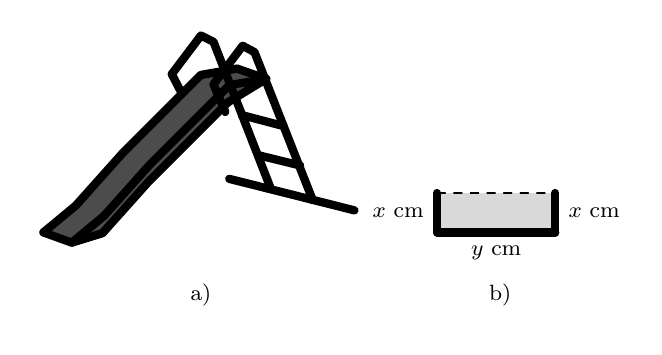
\begin{tikzpicture}[scale=1, font=\footnotesize, line join=round, line cap=round, >=stealth,line width=3.pt]
			\clip(-0.2,-1.2) rectangle (7.5,2.6);
			\fill[line width=3.pt,color=black,fill=black,fill opacity=0.7] (0,0)--(0.41,0.34)--(1,1)--(1.76,1.76)--(2,2)--(2.46,2.08)--(2.83,1.95)--(2.34,1.65)--(1.34,0.65)--(0.75,-0.01)--(0.36,-0.13)-- cycle;
			\draw (0,0)--(0.41,0.34)--(1,1)--(2,2)--(2.46,2.08);
			\draw (0,0)--(0.36,-0.13)--(0.77,0.21)--(0.77,0.21)--(1.36,0.87)--(2.36,1.87)--(2.83,1.95);
			\draw (0.36,-0.13)--(0.75,-0.01)--(1.34,0.65)--(2.34,1.65);
			\draw (2.36,0.68)-- (3.95,0.28);
			\draw (3.42,0.41)--(2.68,2.29)--(2.53,2.37)--(2.16,1.88)--(2.31,1.53);
			\draw (1.63,2.01)--(2,2.5)-- (2.16,2.42)--(2.89,0.55);
			\draw (1.63,2.01)--(1.76,1.76) (2.73,0.98)--(3.26,0.85) (2.52,1.49)--(3.05,1.35);
			\draw (2.34,1.65)--(2.83,1.95)--(2.46,2.08);
			\draw (2,-0.8)node{a)};
			\fill[line width=3.pt,fill=gray,fill opacity=0.3] (5,0.5)--(5,0)--(6.5,0)--(6.5,0.5)--cycle;
			\draw (5,0.5)--(5,0) node [left ,sloped,pos=0.5,rotate=90] {$x$ cm};
			\draw (5,0)--(6.5,0) node [below,sloped,pos=0.5] {$y$ cm};
			\draw (6.5,0)--(6.5,0.5) node [right,sloped,pos=0.5,rotate=-90] {$x$ cm};
			\draw[dashed,thin] (5,0.5)--(6.5,0.5);
			\draw (5.8,-0.8)node{b)};
			%			\draw (4,-1)node{\textit{Hình 5}};
		\end{tikzpicture}
	}
	\loigiai{
		\begin{enumerate}[a)]
			\item Do tấm kim loại có bề rộng $80 \mathrm{~cm}$ nên ta có $2x+y=80 \Leftrightarrow y=80-2x$.\\
			Để có thể thiết kế được máng trượt thì $y>0 \Leftrightarrow 80-2 x>0 \Leftrightarrow x<40$. Suy ra $0<x<40$.\\
			Diện tích của mặt cắt máng trượt là: $S=x y=x(80-2x)=-2x^2+80x$.		
			\item Ta có $S(x)=-2x^2+80x \text{ với } x\in(0; 40)$.
			\allowdisplaybreaks
			\begin{eqnarray*}
				S'(x)&=&-4 x+80 \\
				S'(x)&=&0 \Leftrightarrow-4 x+80=0 \Leftrightarrow x=20.
			\end{eqnarray*}
			Bảng biến thiên của hàm số $S(x)$ như sau
			\begin{center}
				
\begin{tikzpicture}[font=\footnotesize,thick,>=stealth]
					\tikzset{double style/.append style={double distance=1.5pt}}
					\tkzTabInit[nocadre=false,lgt=1.2,espcl=2.5,deltacl=0.6,lw=.75pt]
					{$x$ /0.7, $S'(x)$ /0.8, $S(x)$ /2}
					{$0$,$20$,$40$}
					\tkzTabLine{ ,+,,-, }
					\tkzTabVar{-/$0$,+/$800$,-/$0$}
				\end{tikzpicture}
			\end{center}
			Vậy từ khi $x$ tăng từ $0$ cm đến $20$ cm thì diện tích mặt cắt sẽ tăng dần.
		\end{enumerate}
	}
\end{bt}

% nguồn: 2026-11-16_12_2D1_TL_Ham_so (nhập 16/11/2026)
\begin{bt}%[2D1H1-5]%[ma:d90896d0]
% nguon: Archive/2024/TaiLieuGiangDay/1.HamSo/1. K12 - 4in1 - Hamso/ThubaiGoc/Bai1-Dang5.tex #2674
[SGK12-CTST, Mức độ 2]
	Kim ngạch xuất khẩu rau quả của Việt Nam trong các năm từ $2010$ đến $2017$ có thể được tính xấp xỉ bằng công thức $f(x)=0{,}01x^3-0{,}04x^2+0{,}25x+0{,}44$ (tỉ USD) với $x$ là số năm tính từ $2010$ đến $2017$ $(0\leq x\leq 7)$.
	\begin{flushright}
		(\textit{Theo:} https://infographics.vn/interactive-xuat-khau-rau-qua-
		du-bao-bung-no-dat-4-ty-usd-trong-nam-2023/116220.vna)
	\end{flushright}
	\begin{enumerate}
		\item Tính đạo hàm của hàm số $y=f(x)$.
		\item Chứng minh rằng kim ngạch xuất khẩu rau quả của Việt Nam tăng liên tục trong các năm từ $2010$ đến $2017$.
	\end{enumerate}
	\loigiai{
		\begin{enumerate}
			\item Ta có $f'(x)=0{,}03x^2-0{,}08x+0{,}25$.
			\item Xét $f'(x)=0 \Leftrightarrow 0{,}03x^2-0{,}08x+0{,}25=0$ (vô nghiệm).\\
			Bảng biến thiên
			\begin{center}
				
\begin{tikzpicture}
					\tkzTabInit[nocadre=false,lgt=1.2,espcl=5,deltacl=0.6]
					{$x$ /0.6,$f'(x)$ /0.6,$f(x)$ /2}
					{$0$,$7$}
					\tkzTabLine{,+,}
					\tkzTabVar{-/$0{,}44$,+/$3{,}66$}
				\end{tikzpicture}
			\end{center}
			Từ bảng biến thiên trên, ta thấy $f'(x)>0$, $\forall x\in [0;7]$.\\
			Vậy kim ngạch xuất khẩu rau quả của Việt Nam tăng liên tục trong các năm từ $2010$ đến $2017$.
		\end{enumerate}
	}
\end{bt}

% nguồn: 2026-11-16_12_2D1_TL_Ham_so (nhập 16/11/2026)
\begin{bt}%[2D1H1-5]%[ma:90a331ec]
% nguon: Archive/2024/TaiLieuGiangDay/1.HamSo/1. K12 - 4in1 - Hamso/ThubaiGoc/Bai1-Dang5.tex #2678
[Mức độ 2]%
	Định luật Moore được xây dựng bởi Gordon More-một trong những sáng lập viên của tập đoàn sản xuất chip máy tính nổi tiếng Intel. Định luật ban đầu được phát biểu như sau
	\lq\lq Số lượng transistor trên mỗi đơn vị inch vuông sẽ tăng lên gấp đôi sau mỗi $24$ tháng. \rq\rq ($1$ inch vuông xấp xỉ $6{,}45$ cm$^2$).
	Phương trình sau đây mô tả định luật Moore
	$$n_i=n_0\cdot 2^{\tfrac{y_i-y_0}{2}}$$
	trong đó $n_0$ là số lượng transitor trên một đơn vị diện tích ban đầu, $y_0$ là năm ứng với $n_0$, $n_i$ là số lượng transitor tại năm $y_i$ đang xét. \\
	(Nguồn: https://scipython.com/book/chapter-3-simple-plotting-with-pylab/examples/moores-law/)\\
	Nhận xét về tính đơn điệu của hàm số mô tả định luật Moore.
	\loigiai{
		Xét hàm số $n_i=n_0\cdot 2^{\tfrac{y_i-y_0}{2}}$.\\
		Ta có $n_i'=n_0\cdot 2^{\tfrac{y_i-y_0}{2}}\cdot \ln 2>0~\forall y_i$.\\
		Suy ra hàm số đồng biến.
	}
\end{bt}

% nguồn: 2026-11-16_12_2D1_TL_Ham_so (nhập 16/11/2026)
% nguồn: 2026-11-16_12_2D1_TL_Ham_so (nhập 16/11/2026)
\begin{bt}%[2D1H1-5]%[ma:80ff739a]
% nguon: Archive/2024/TaiLieuGiangDay/1.HamSo/1. K12 - 4in1 - Hamso/ThubaiGoc/Bai1-Dang5.tex #2680
[SGK12-KNTT, Mức độ 2]%[BG12-4in1, Trần Thiên Đức]
	Xét một chất điểm chuyển động trên một trục số nằm ngang, chiều dương từ trái sang phải (Hình vẽ). Giả sử vị trí $s(t)$ (mét) của chất điểm trên trục số đã chọn tại thời điểm $t$ (giây) được cho bởi công thức
	\[s(t)=t^3-9t^2+15t,\,\, t\ge 0.\]
	Hỏi trong khoảng thời gian nào thì chất điểm chuyển động sang phải, trong khoảng thời gian nào  thì chất điểm chuyển động sang trái?
	\begin{center}
		\begin{tikzpicture}[>=stealth,line join=round,line cap=round,font=\footnotesize,scale=1]
			\draw[->] (0,0)coordinate (O)--(5,0)coordinate (B);
			\draw[thick] 
			(1.5,-.05)--(1.5,.05)node[below=1mm,black]{$O$}
			(3,-.05)--(3,.05)node[below=1mm,black]{$s(t)$}
			;
			\path 
			(O)--(B)node[midway,below=6mm,orange]{}
			;
		\end{tikzpicture}
	\end{center}
	\loigiai{
		Theo ý nghĩa cơ học của đạo hàm, vận tốc $v\left(t\right)$ là đạo hàm của $s\left(t\right)$. \\
		Ta có $v\left(t\right) = s'\left(t\right) = \left(t^3 -9t^2 + 15t\right)' = 3t^2 - 18t + 15$.\\
		Tập xác định $\mathscr{D} = \mathbb{R}$.\\
		Ta có $v(t)=0\Leftrightarrow\hoac{&t=1 \\&t=5. }$\\
		Bảng xét dấu
		\begin{center}
			
\begin{tikzpicture}[scale=1, font=\footnotesize]
				\tkzTabInit[nocadre=false, lgt=1.2, espcl=2, deltacl=0.6]
				{$t$/0.6,$v(t)$/0.6}
				{$-\infty$,$1$,$5$,$+\infty$};
				\tkzTabLine{,+,$0$,-,$0$,+,};
			\end{tikzpicture}
		\end{center}
		Chất điểm chuyển động theo chiều dương (sang bên phải) khi $v\left(t\right) > 0$, tức là $t \in \left(-\infty; 1\right) \cup \left(5; +\infty\right)$.\\
		Chất điểm chuyển động theo chiều âm (sang bên trái) khi $v\left(t\right) < 0$, tức là $1 < t < 5$.
	}	
\end{bt}

% nguồn: 2026-11-16_12_2D1_TL_Ham_so (nhập 16/11/2026)
\begin{bt}%[2D1H1-5]%[ma:fe2d157b]
% nguon: Archive/2024/TaiLieuGiangDay/1.HamSo/1. K12 - 4in1 - Hamso/ThubaiGoc/Bai1-Dang5.tex #2681
[Mức độ 2]
	Một vật được phóng thẳng đứng lên trên từ độ cao $2 \mathrm{~m}$ với vận tốc ban đầu là $24{,}5 \mathrm{~m} / \mathrm{s}$. Trong Vật lí, ta biết rằng khi bỏ qua sức cản của không khí thì độ cao $h$ (mét) của vật sau $t$ (giây) được cho bởi công thức
	$$
	h(t)=2+24{,}5 t-4{,}9t^{2}.
	$$
	Hỏi tại từ thời điểm $t=3$ (giây) đến $t=4$ (giây), thì độ cao của vật tăng hay giảm?
	\loigiai{
		Xét hàm số $h(t)=2+24{,}5 t-4{,}9t^{2}$ với $t>0$.\\
		Ta có $h'(t)=24{,}5-9{,}8t$. \\
		$h'(t)=0\Leftrightarrow t=2{,}5$. \\
		Lập bảng biến thiên của $h(t)$: 
		\begin{center}
			
\begin{tikzpicture}
				\tkzTabInit[nocadre=false,lgt=1.2,espcl=3.5,deltacl=0.6]
				{$t$ /0.6,$h'(t)$ /0.6,$h(t)$ /1.4}
				{$0$,$2{,}5$,$+\infty$}
				\tkzTabLine{,+,0,-,}
				\tkzTabVar{-/,+/$32{,}625$,-/}
			\end{tikzpicture}
		\end{center}
		Từ bảng biến thiên ta suy ra từ thời điểm $t=3$ (giây) đến $t=4$ (giây), thì độ cao của vật giảm.
	}
\end{bt}

% nguồn: 2026-11-16_12_2D1_TL_Ham_so (nhập 16/11/2026)
\begin{bt}%[2D1V1-5]%[ma:0870a7d1]
% nguon: Archive/2024/TaiLieuGiangDay/1.HamSo/1. K12 - 4in1 - Hamso/ThubaiGoc/Bai1-Dang5.tex #2682
[Mức độ 3]%
	Giả sử dân số của một thị trấn sau $t$ năm kể từ năm $2000$ được mô tả bởi hàm số $$N\left(t\right)=\frac{25t+10}{t+5}, t\ge0,$$
	trong đó $N\left(t\right)$ được tính bằng nghìn người. Tính đạo hàm $N^\prime\left(t\right)$ và $\lim\limits_{t \to +\infty}N\left(t\right)$. Từ đó giải thích tại sao dân số của thị trấn đó luôn tăng nhưng sẽ không vượt quá một ngưỡng nào đó.
	\loigiai{
		Xét hàm số  $N\left(t\right)=\dfrac{25t+10}{t+5}, t\ge0$.\\
		Ta có $N^\prime\left(t\right)=\dfrac{115}{\left(t+5\right)^2}$.\\
		$\lim\limits_{t \to +\infty}N\left(t\right)=\lim\limits_{t \to +\infty}\dfrac{25t+10}{t+5}=25$.\\
		Bảng biến thiên của hàm số như sau
		\begin{center}
			
\begin{tikzpicture}[font=\footnotesize,thick,>=stealth]
				\tikzset{double style/.append style={double distance=1.5pt}}
				\tkzTabInit[nocadre=false,lgt=1.2,espcl=2.5,deltacl=0.6,lw=.75pt]
				{$x$ /0.6,$y'$ /0.6,$y$ /2.5}
				{$-\infty$,$-5$,$+\infty$}
				\tkzTabLine{,+,d,+,}
				\tkzTabVar{-/$25$,+D-/$+\infty$/$-\infty$,+/$25$}
			\end{tikzpicture}
		\end{center}
		Từ bảng biến thiên ta có dân số của thị trấn đó luôn tăng nhưng sẽ không vượt quá $25$ ngàn người.
	}
\end{bt}

% nguồn: 2026-11-16_12_2D1_TL_Ham_so (nhập 16/11/2026)
% nguồn: 2026-11-16_12_2D1_TL_Ham_so (nhập 16/11/2026)
\begin{bt}%[2D1H1-5]%[ma:4d0727a5]
% nguon: Archive/2024/TaiLieuGiangDay/1.HamSo/1. K12 - 4in1 - Hamso/Thubai/Bai1-Dang5.tex #3042
%%[SGK12 - Cánh Diều, Mức độ 2]
	\immini{
		Máng trượt của một cầu trượt cho trẻ em (\textit{Hình a}) được uốn từ một tấm kim loại có bề rộng $80$ cm, mặt cắt được mô tả ở \textit{Hình b}. Nhà thiết kế khuyến cáo, diện tích mặt cắt càng lớn thì càng đảm bảo an toàn cho trẻ em.
		\begin{enumerate}[a)]
			\item Gọi $S$ là diện tích mặt cắt. Tìm điều kiện của $x$ và viết công thức tính $S$ theo $x$.
			\item Diện tích mặt cắt sẽ tăng hay giảm khi chúng ta tăng giá trị của $x$ từ 0 cm đến 10 cm?
		\end{enumerate}
	}{
		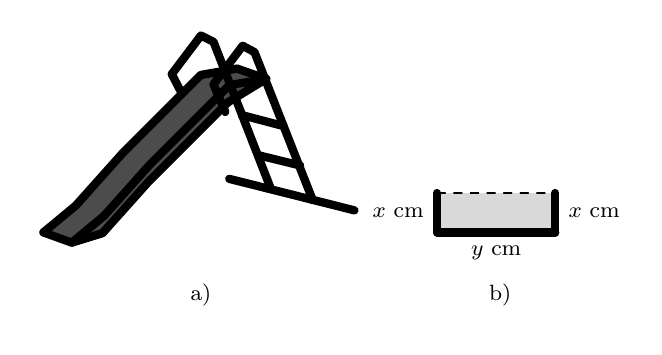
\begin{tikzpicture}[scale=1, font=\footnotesize, line join=round, line cap=round, >=stealth,line width=3.pt]
			\clip(-0.2,-1.2) rectangle (7.5,2.6);
			\fill[line width=3.pt,color=black,fill=black,fill opacity=0.7] (0,0)--(0.41,0.34)--(1,1)--(1.76,1.76)--(2,2)--(2.46,2.08)--(2.83,1.95)--(2.34,1.65)--(1.34,0.65)--(0.75,-0.01)--(0.36,-0.13)-- cycle;
			\draw (0,0)--(0.41,0.34)--(1,1)--(2,2)--(2.46,2.08);
			\draw (0,0)--(0.36,-0.13)--(0.77,0.21)--(0.77,0.21)--(1.36,0.87)--(2.36,1.87)--(2.83,1.95);
			\draw (0.36,-0.13)--(0.75,-0.01)--(1.34,0.65)--(2.34,1.65);
			\draw (2.36,0.68)-- (3.95,0.28);
			\draw (3.42,0.41)--(2.68,2.29)--(2.53,2.37)--(2.16,1.88)--(2.31,1.53);
			\draw (1.63,2.01)--(2,2.5)-- (2.16,2.42)--(2.89,0.55);
			\draw (1.63,2.01)--(1.76,1.76) (2.73,0.98)--(3.26,0.85) (2.52,1.49)--(3.05,1.35);
			\draw (2.34,1.65)--(2.83,1.95)--(2.46,2.08);
			\draw (2,-0.8)node{a)};
			\fill[line width=3.pt,fill=gray,fill opacity=0.3] (5,0.5)--(5,0)--(6.5,0)--(6.5,0.5)--cycle;
			\draw (5,0.5)--(5,0) node [left ,sloped,pos=0.5,rotate=90] {$x$ cm};
			\draw (5,0)--(6.5,0) node [below,sloped,pos=0.5] {$y$ cm};
			\draw (6.5,0)--(6.5,0.5) node [right,sloped,pos=0.5,rotate=-90] {$x$ cm};
			\draw[dashed,thin] (5,0.5)--(6.5,0.5);
			\draw (5.8,-0.8)node{b)};
			%			\draw (4,-1)node{\textit{Hình 5}};
		\end{tikzpicture}
	}
	\loigiai{
		\begin{enumerate}[a)]
			\item Do tấm kim loại có bề rộng $80 \mathrm{~cm}$ nên ta có $2x+y=80 \Leftrightarrow y=80-2x$.\\
			Để có thể thiết kế được máng trượt thì $y>0 \Leftrightarrow 80-2 x>0 \Leftrightarrow x<40$. Suy ra $0<x<40$.\\
			Diện tích của mặt cắt máng trượt là: $S=x y=x(80-2x)=-2x^2+80x$.		
			\item Ta có $S(x)=-2x^2+80x \text{ với } x\in(0; 40)$.
			\allowdisplaybreaks
			\begin{eqnarray*}
				S'(x)&=&-4 x+80 \\
				S'(x)&=&0 \Leftrightarrow-4 x+80=0 \Leftrightarrow x=20.
			\end{eqnarray*}
			Bảng biến thiên của hàm số $S(x)$ như sau
			\begin{center}
				
\begin{tikzpicture}[font=\footnotesize,thick,>=stealth]
					\tikzset{double style/.append style={double distance=1.5pt}}
					\tkzTabInit[nocadre=false,lgt=1.2,espcl=2.5,deltacl=0.6,lw=.75pt]
					{$x$ /0.7, $S'(x)$ /0.8, $S(x)$ /2}
					{$0$,$20$,$40$}
					\tkzTabLine{ ,+,,-, }
					\tkzTabVar{-/$0$,+/$800$,-/$0$}
				\end{tikzpicture}
			\end{center}
			Vậy từ khi $x$ tăng từ $0$ cm đến $20$ cm thì diện tích mặt cắt sẽ tăng dần.
		\end{enumerate}
	}
\end{bt}

% nguồn: 2026-11-16_12_2D1_TL_Ham_so (nhập 16/11/2026)
\begin{bt}%[2D1H1-5]%[ma:bf82a3e3]
% nguon: Archive/2024/TaiLieuGiangDay/1.HamSo/1. K12 - 4in1 - Hamso/Thubai/Bai1-Dang5.tex #3044
%%[SGK12-CTST, Mức độ 2]
	Kim ngạch xuất khẩu rau quả của Việt Nam trong các năm từ $2010$ đến $2017$ có thể được tính xấp xỉ bằng công thức $f(x)=0{,}01x^3-0{,}04x^2+0{,}25x+0{,}44$ (tỉ USD) với $x$ là số năm tính từ $2010$ đến $2017$ $(0\leq x\leq 7)$.
	\begin{flushright}
		(\textit{Theo:} https://infographics.vn/interactive-xuat-khau-rau-qua-
		du-bao-bung-no-dat-4-ty-usd-trong-nam-2023/116220.vna)
	\end{flushright}
	\begin{enumerate}
		\item Tính đạo hàm của hàm số $y=f(x)$.
		\item Chứng minh rằng kim ngạch xuất khẩu rau quả của Việt Nam tăng liên tục trong các năm từ $2010$ đến $2017$.
	\end{enumerate}
	\loigiai{
		\begin{enumerate}
			\item Ta có $f'(x)=0{,}03x^2-0{,}08x+0{,}25$.
			\item Xét $f'(x)=0 \Leftrightarrow 0{,}03x^2-0{,}08x+0{,}25=0$ (vô nghiệm).\\
			Bảng biến thiên
			\begin{center}
				
\begin{tikzpicture}
					\tkzTabInit[nocadre=false,lgt=1.2,espcl=5,deltacl=0.6]
					{$x$ /0.6,$f'(x)$ /0.6,$f(x)$ /2}
					{$0$,$7$}
					\tkzTabLine{,+,}
					\tkzTabVar{-/$0{,}44$,+/$3{,}66$}
				\end{tikzpicture}
			\end{center}
			Từ bảng biến thiên trên, ta thấy $f'(x)>0$, $\forall x\in [0;7]$.\\
			Vậy kim ngạch xuất khẩu rau quả của Việt Nam tăng liên tục trong các năm từ $2010$ đến $2017$.
		\end{enumerate}
	}
\end{bt}

% nguồn: 2026-11-16_12_2D1_TL_Ham_so (nhập 16/11/2026)
\begin{bt}%[2D1H1-5]%[ma:d42b7b45]
% nguon: Archive/2024/TaiLieuGiangDay/1.HamSo/1. K12 - 4in1 - Hamso/Thubai/Bai1-Dang5.tex #3048
%%[Mức độ 2]%
	Định luật Moore được xây dựng bởi Gordon More-một trong những sáng lập viên của tập đoàn sản xuất chip máy tính nổi tiếng Intel. Định luật ban đầu được phát biểu như sau
	\lq\lq Số lượng transistor trên mỗi đơn vị inch vuông sẽ tăng lên gấp đôi sau mỗi $24$ tháng. \rq\rq ($1$ inch vuông xấp xỉ $6{,}45$ cm$^2$).
	Phương trình sau đây mô tả định luật Moore
	$$n_i=n_0\cdot 2^{\tfrac{y_i-y_0}{2}}$$
	trong đó $n_0$ là số lượng transitor trên một đơn vị diện tích ban đầu, $y_0$ là năm ứng với $n_0$, $n_i$ là số lượng transitor tại năm $y_i$ đang xét. \\
	(Nguồn: https://scipython.com/book/chapter-3-simple-plotting-with-pylab/examples/moores-law/)\\
	Nhận xét về tính đơn điệu của hàm số mô tả định luật Moore.
	\loigiai{
		Xét hàm số $n_i=n_0\cdot 2^{\tfrac{y_i-y_0}{2}}$.\\
		Ta có $n_i'=n_0\cdot 2^{\tfrac{y_i-y_0}{2}}\cdot \ln 2>0~\forall y_i$.\\
		Suy ra hàm số đồng biến.
	}
\end{bt}

% nguồn: 2026-11-16_12_2D1_TL_Ham_so (nhập 16/11/2026)
\begin{bt}%[2D1H1-5]%[ma:b94270b7]
% nguon: Archive/2024/TaiLieuGiangDay/1.HamSo/1. K12 - 4in1 - Hamso/Thubai/Bai1-Dang5.tex #3049
%%[SGK12-KNTT, Mức độ 2]%[BG12-4in1, Trần Thiên Đức]
	Xét một chất điểm chuyển động trên một trục số nằm ngang, chiều dương từ trái sang phải (Hình vẽ). Giả sử vị trí $s(t)$ (mét) của chất điểm trên trục số đã chọn tại thời điểm $t$ (giây) được cho bởi công thức
	\[s(t)=t^3-9t^2+15t,\,\, t\ge 0.\]
	Hỏi trong khoảng thời gian nào thì chất điểm chuyển động sang phải, trong khoảng thời gian nào  thì chất điểm chuyển động sang trái?
	\begin{center}
		\begin{tikzpicture}[>=stealth,line join=round,line cap=round,font=\footnotesize,scale=1]
			\draw[->] (0,0)coordinate (O)--(5,0)coordinate (B);
			\draw[thick] 
			(1.5,-.05)--(1.5,.05)node[below=1mm,black]{$O$}
			(3,-.05)--(3,.05)node[below=1mm,black]{$s(t)$}
			;
			\path 
			(O)--(B)node[midway,below=6mm,orange]{}
			;
		\end{tikzpicture}
	\end{center}
	\loigiai{
		Theo ý nghĩa cơ học của đạo hàm, vận tốc $v\left(t\right)$ là đạo hàm của $s\left(t\right)$. \\
		Ta có $v\left(t\right) = s'\left(t\right) = \left(t^3 -9t^2 + 15t\right)' = 3t^2 - 18t + 15$.\\
		Tập xác định $\mathscr{D} = \mathbb{R}$.\\
		Ta có $v(t)=0\Leftrightarrow\hoac{&t=1 \\&t=5. }$\\
		Bảng xét dấu
		\begin{center}
			
\begin{tikzpicture}[scale=1, font=\footnotesize]
				\tkzTabInit[nocadre=false, lgt=1.2, espcl=2, deltacl=0.6]
				{$t$/0.6,$v(t)$/0.6}
				{$-\infty$,$1$,$5$,$+\infty$};
				\tkzTabLine{,+,$0$,-,$0$,+,};
			\end{tikzpicture}
		\end{center}
		Chất điểm chuyển động theo chiều dương (sang bên phải) khi $v\left(t\right) > 0$, tức là $t \in \left(-\infty; 1\right) \cup \left(5; +\infty\right)$.\\
		Chất điểm chuyển động theo chiều âm (sang bên trái) khi $v\left(t\right) < 0$, tức là $1 < t < 5$.
	}	
\end{bt}

% nguồn: 2026-11-16_12_2D1_TT_Ham_so (nhập 16/11/2026)
% nguồn: 2026-11-16_12_2D1_TT_Ham_so (nhập 16/11/2026)
\begin{bt}%[2D1H1-5]%[ma:909bfb27]
% nguon: Archive/SP_SauLuoi_2024-2025/SP_HKI/2-TN-DS-TLN-THPT-DinhTienHoang-NinhBinh-HKI-NH24-25.tex #97
%[Dự án đề kiểm tra Khối 12 HK1 NH24-25 - Đợt 4 - Đắc Vũ]%[THPT Đinh Tiên Hoàng - Tỉnh Ninh Bình] 
	Kính viễn vọng không gian Hubble được đưa vào vũ trụ ngày 24/4/1990 bằng tàu con thoi Discovery. Vận tốc của tàu con thoi trong sứ mệnh này, từ lúc cất cánh tại thời điểm $t=0$ (s) cho đến khi tên lửa đẩy được phóng đi tại thời điểm $t=126$ (s), được cho bởi hàm số:  $v(t)=0{,}001302 t^3-0{,}09029 t^2+23$, (vận tốc $v$ được tính bằng ft/s, $1$ feet $= 0{,}3048$ m).  Gia tốc của tàu con thoi sẽ tăng từ giây thứ bao nhiêu (làm tròn đến hàng đơn vị), tính từ thời điểm $t=0$ (s), cho đến khi tên lửa đẩy được phóng đi?
	\shortans{23}
	\loigiai{
		Gia tốc là đạo hàm của vận tốc, tức là
		$$a(t)=v'(t)=0{,}003906t^2-0{,}18058t.$$
		Xét hàm số $a(t)=0{,}003906t^2-0{,}18058t$ với $t \in [0;126]$.\\		
		Đạo hàm của $a(t)$ là
		$$a'(t)=0{,}007812t-0{,}18058$$		
		Phương trình $a'(t)=0 \Leftrightarrow 0{,}006192t-0{,}18058=0 \Leftrightarrow t\approx 23{,}11$.\\
		Bảng biến thiên
		\begin{center}
			
\begin{tikzpicture}[font=\footnotesize, line join=round,line cap=round, >=stealth]
				\tkzTabInit[nocadre=false,lgt=1.2,espcl=2.5,deltacl=0.6]
				{$x$ /0.6,$y’$ /0.6,$y$ /2}
				{$0$,$23{,}11$, $126$}
				\tkzTabLine{,-,0,+,}
				\tkzTabVar{+/ $23$,-/ $1{,}905$,+/ $61{,}83$}
			\end{tikzpicture}
		\end{center}
		Vậy gia tốc của tàu con thoi tăng từ thời điểm $t=23$ (kết quả làm tròn đến hàng đơn vị).
	}
\end{bt}

% nguồn: 2026-11-16_12_2D1_TT_Ham_so (nhập 16/11/2026)
\begin{ex}%[2D1V1-5]%[ma:fd33a1ed]
% nguon: Archive/SP_SauLuoi_2024-2025/SP_HKI/2-TL-TN-DS-TLN-ChuyenLeQuyDon-DaNang-HKI-NH24-25.tex #103
%[Lớp 12- Kiểm tra giữa học kỳ - THPT Chuyên Lê Quý Đôn - Đà Nẵng]%[Nguyễn Văn Sang]
	Trong $25$ phút theo dõi, lưu lượng nước của một con sông được tính theo công thức
	$$
	Q(t)=-\dfrac{t^3}{10}+5 t^2+50.
	$$
	Trong đó $Q$ tính theo $\mathrm{m}^3/$ phút, $t$ tính theo phút, $0 \leq t \leq 25$. Khi lưu lượng nước của con sông lên đến $500 \mathrm{~m}^3 / \mathrm{phút}$ thì cảnh báo lũ được đưa ra.
	\choiceTF
	{\True Lưu lượng nước sông lúc bắt đầu theo dõi là $50 \mathrm{~m}^3 /$ phút}
	{Cảnh báo lũ được đưa ra trước thời điểm $t=10$ phút}
	{Trong khoảng thời gian $10$ phút đầu tiên, không có thời điểm nào mà tốc độ tăng của lưu lượng nước sông bằng $40 \mathrm{~m}^3/(\text{phút})^2$}
	{\True Trong khoảng thời gian từ phút thứ $10$ đến phút thứ $15$, lưu lượng nước sông trung bình mỗi phút tăng $77{,}5 \mathrm{~m}^3 /$ phút}
	\loigiai{
	 \begin{itemchoice}
	 \itemch \textbf{Đúng} vì\\
	Khi $t = 0$, ta có
		 $$
		 Q(0) = -\dfrac{0^3}{10} + 5 \cdot 0^2 + 50 = 50 \mathrm{~m}^3/\text{phút}.
		 $$
	 \itemch \textbf{Sai} vì\\
	 Xét hàm số $Q(t)=-\dfrac{t^3}{10}+5 t^2+50$, có $Q'(t)=-\dfrac{3t^2}{10}+10t$.\\
	 Cho $Q'(t)=0\Leftrightarrow \hoac{&t=0 & (\text{nhận vì } t\in \left[0;25\right])\\&t=\dfrac{100}{3}&(\text{loại vì } t\in \left[0;25\right]).}$\\
	Bảng biến thiên
	\begin{center}
		\begin{tikzpicture}[scale=1, font=\footnotesize, line join=round, line cap=round, >=stealth]
			\tkzTabInit[nocadre=false,lgt=1.25,espcl=2,deltacl=0.75]
			{$t$/.7 ,$Q'(t)$/.7,$Q(t)$/2}
			{$0$,$ $ , $25$}
			\draw[dashed,->](3,-.57)node[above] {$10$}--(3,-2.75)node[below] {$450$};
			\tkzTabLine{ ,  , + , , }

			\draw[->] (2,-3.13)node[left] {$50$} -- (5.5,-1.75)node[right] {$1612{,}5$};
		\end{tikzpicture}
	\end{center}
	Dựa vào bảng biến thiên, $10$ phút đầu tiên lưu lượng nước chưa đạt mức cảnh báo là $500 \mathrm{~m}^3 / \mathrm{phút}$.
	 \itemch \textbf{Sai} vì
	 \begin{itemize}
		\item Hàm tốc độ thay đổi của lưu lượng nước là đạo hàm của $Q(t)$, ta có
		$$
		Q'(t) = -\dfrac{3t^2}{10} + 10t, \mathrm{~m}^3/(\text{phút})^2.
		$$
		\item Giải phương trình $Q'(t) = 40$ ta có 
		$$
		-\dfrac{3t^2}{10} + 10t = 40 \Leftrightarrow
		-3t^2 + 100t - 400 = 0 \Leftrightarrow \hoac{&t \approx 28{,}68 &(\text{loại vì } t \leq 25)\\&t\approx 4{,}65 &(\text{nhận vì } 0\leq t \leq 25).}
		$$
		\item Nhận thấy $t \approx 4{,}65$ thuộc khoảng $10$ phút đầu, nên tồn tại thời điểm trong $10$ phút đầu mà $Q'(t) = 40 \mathrm{~m}^3/(\text{phút})^2$.
	\end{itemize}
	 \itemch \textbf{Đúng} vì
	 \begin{itemize}
		\item Tính lưu lượng tại $t = 10$ và $t = 15$, ta có\\
		$
		Q(10) = -\dfrac{1000}{10} + 5 \cdot 100 + 50 = -100 + 500 + 50 = 450 \mathrm{~m}^3/\text{phút}.
		$\\ 
		$
		Q(15) = -\dfrac{3375}{10} + 5 \cdot225 + 50 = -337{,}5 + 1125 + 50 = 837{,}5 \mathrm{~m}^3/\text{phút}.
		$
		\item Lưu lượng trung bình $Q_{\text{trung bình}}$ trong khoảng $t$ từ $10$ đến $15$:
		$$
		Q_{\text{trung bình}} = \dfrac{Q(15) - Q(10)}{15 - 10} = \dfrac{837{,}5 - 450}{5} = \dfrac{387{,}5}{5} = 77{,}5 \mathrm{~m}^3/\text{phút}.
		$$
	\end{itemize}
	 \end{itemchoice}
	}
\end{ex}

% nguồn: 2026-11-16_12_2D1_TT_Ham_so (nhập 16/11/2026)
\begin{bt}%[2D1V1-5]%[ma:2b36c4c4]
% nguon: Archive/SP_SauLuoi_2024-2025/SP_HKI/2-TN-DS-TLN-THPT-GiaDinh-TPHCM-HKI-NH24-25.tex #141
%[Dự án A đợt 5,Nguyễn Tài Tuệ]%[THPT Gia Định, TPHCM]
	Quan sát một đàn ong trong $20$ tuần, người ta ước lượng được số lượng ong trong đàn bởi công thức $P(t)=\dfrac{20\,000}{1+10\,000 \mathrm{e}^{-t}}$, trong đó $t$ là thời gian tính theo tuần kể từ khi bắt đầu quan sát, $0 \leq t \leq 20$. Tại thời điểm nào thì số lượng ong của đàn tăng nhanh nhất (kết quả làm tròn đến hàng đơn vị của tuần).\par
	\shortans{$9$}
	\loigiai{
		Tốc độ thay đổi số lượng ong của đàn theo thời gian $t$ là		
		$$
		T(t)=P'(t)=2 \cdot 10^8 \cdot \dfrac{\mathrm{e}^{-t}}{\left(1+10\,000 \mathrm{e}^{-t}\right)^2}
		$$
		
		
		Ta có 
		\begin{eqnarray*}
			T'(t)&=&2 \cdot 10^8 \cdot \dfrac{-\mathrm{e}^{-t}\cdot\left(1+10\,000 \mathrm{e}^{-t}\right)^2-\mathrm{e}^{-t}\cdot 2 \cdot\left(1+10\,000 \mathrm{e}^{-t}\right) \cdot\left(-10\,000 \mathrm{e}^{-t}\right)}{\left(1+10\,000 \mathrm{e}^{-t}\right)^4}\\
			&=&2 \cdot 10^8 \cdot \dfrac{\mathrm{e}^{-t}\cdot\left(10\,000 \mathrm{e}^{-t}-1\right)}{\left(1+10\,000 \mathrm{e}^{-t}\right)^3}.
		\end{eqnarray*}
		
		$$T'(t)=0 \Leftrightarrow 10\,000-\mathrm{e}^t=0 \Leftrightarrow t=\ln 10\,000.$$
		
		Bảng xét dấu của đạo hàm
		\begin{center}
			
\begin{tikzpicture}
				\tkzTabInit[lgt=1.2,espcl=2]
				{$x$/0.7,$T’(x)$/.7 }
				{$0$,$\ln 10\,000$,$20$}
				\tkzTabLine{ ,+,z,-, }	 	 
			\end{tikzpicture}
		\end{center}	
		Từ đó, $T(t)$ đạt giá trị lớn nhất tại $t=\ln 10\,000 \approx 9$.\\
		Vậy đàn ong tăng nhanh nhất tại thời điểm khoảng $t=9$ tuần.}
\end{bt}

% nguồn: 2026-11-16_12_2D1_TT_Ham_so (nhập 16/11/2026)
% nguồn: 2026-11-16_12_2D1_TT_Ham_so (nhập 16/11/2026)
% nguồn: 2026-11-16_12_2D1_TT_Ham_so (nhập 16/11/2026)
\begin{bt}%[2D1H1-5]%[ma:11c5e359]
% nguon: Archive/SP_SauLuoi_2024-2025/SP_GHKI/2-TL-TN-TLN-THPT-PhamVanSang-HCM-GHKI-NH24-25€.tex #205
%[CTST - Lớp 12 - Đề chính thức - THPT Phạm Văn Sáng - TPHCM]%[Hiếu Mai]
	Kính viễn vọng không gian Hubble được đưa vào vũ trụ ngày 24/4/1990 bằng tàu con thoi Discovery.
	Vận tốc của tàu con thoi trong sứ mệnh này, từ lúc cất cánh tại thời điểm $t=0~(\text{s})$ cho đến khi tên lửa đẩy được phóng đi tại thời điểm $t=126~(\text{s})$, được cho bởi hàm số sau
	$v(t) = 0{,}001302t^3 - 0{,}09029t^2+23$,
	($v(t)$ được tính bằng $\text{feet}/\text{s}$, $1~\text{feet} = 0{,}3048~\text{m}$).
	(\textit{Nguồn: J. Stewart, Calculus Seventh Edition, Brooks/Cole, CENGAGE Learning 2012}).
	Gia tốc của tàu con thoi được tính bằng công thức $a(t)=v'(t)$ sẽ tăng trong khoảng thời gian $(a,b)$ đơn vị (s) tính từ thời điểm cất cánh cho đến khi tên lửa đẩy được phóng đi.
	Tính $a+b$ (quy tròn đến hàng đơn vị).
	\shortans{$149$}
	\loigiai{
		Trong khoảng thời gian $t=0$ đến $t=126~\text{s}$, vận tốc của tên lửa là
		$$
		v(t) = 0{,}001302t^3 - 0{,}09029t^2+23.
		$$
		Do đó gia tốc của nó là
		$$
		a(t)
		= v'(t)
		= 0{,}003906 t^2 - 0{,}18058 t.
		$$
		Xét đạo hàm của gia tốc
		$$
		a'(t)
		= 0{,}007812 t - 0{,}18058.
		$$
		Cho $a'(t)=0$, ta được
		$$
		0{,}007812 t - 0{,}18058
		\Rightarrow
		t \approx 23~\text{s}.
		$$
		Lập bảng biến thiên của $a(t)$:
		\begin{center}
			
\begin{tikzpicture}
				\tkzTabInit[lgt=2,espcl=3]
				{$t$/1, $a'(t)$/1, $t$/2}
				{$0$, $23$, $126$}
				\tkzTabLine{, -, z, +}
				\tkzTabVar{+/$a(0)$, -/$a(23)$, +/$a(126)$}
			\end{tikzpicture}
		\end{center}
		Dựa vào bảng biến thiên trên, ta thấy $a(t)$ tăng trong khoảng $(23;126)$. 
		\\
		Do đó $a=23$ và $b=126$.
		\\
		Vậy $a+b=149$.
	}
\end{bt}

% nguồn: 2026-11-16_12_2D1_TT_Ham_so (nhập 16/11/2026)
\begin{bt}%[2D1V1-5]%[ma:5048b2c4]
% nguon: Archive/SP_SauLuoi_2024-2025/SP_GHKI/2-TN-DS-TLN-THPT-Nguyen-Thai-Binh-TPHCM-GHKI-NH23-24.tex #233
%[2-THPT-NguyenThaiBinh-GHKI-NH24-25]%[Nguyễn Đức Lợi]
	Thể tích $V$(cm$^3$) của $1$kg nước tại nhiệt độ $T, (0^\circ C \le T  \le 30^\circ C)$ được tính bởi công thức $V(T) = 999{,}87 - 0{,}06426 T + 0{,}0085043 T^2 - 0{,}0000679 T^3$. Thể tích nước $V(T),  (0^\circ C \le T  \le 30^\circ C)$ tăng trong khoảng nhiệt độ $(a^\circ; b^\circ)$, với $a$, $b$ là các số nguyên dương. Tổng $a+ b$ bằng bao nhiêu? (Kết quả được làm tròn đến hàng đơn vị).
	\shortans{34}	
	\loigiai{
	Ta có $V'(T) = - 0{,}06426 + 0{,}0170086 T - 0{,}0002037 T^2$.\\
	Xét phương trình $V'(T) = 0 \Leftrightarrow - 0{,}06426 + 0{,}0170086 T - 0{,}0002037 T^2 = 0 \Leftrightarrow \hoac{&T =T_1 \approx 4 \\ & T = T_2 \approx 80.}$\\
	Suy ra bảng biến thiên của $V(T)$ trên đoạn $[0; 30]$ như sau:
	\begin{center}
	
\begin{tikzpicture}
\tkzTabInit[espcl=4,lgt=2,nocadre]
{$T$/0.7,$V'(T)$/0.7,$V(T)$/2.1}
{$0$,$T_1$,$30$}
\tkzTabLine{,-,0,+,}
\tkzTabVar{+/$V(0)$,-/$V(T_1)$,+/$V(30)$}
\end{tikzpicture}
	\end{center}
	Từ bảng biến thiên ta thấy $V(T)$ tăng trong khoảng từ $(T_1;30)$.\\
	Suy ra $a = 4; b = 30$.\\
	Vậy $a + b = 4 + 30 = 34$.
	}
\end{bt}

% nguồn: 2026-11-16_12_2D1_TT_Ham_so (nhập 16/11/2026)
\begin{bt}%[2D1V1-5]%[ma:93f755d2]
% nguon: Archive/SP_SauLuoi_2024-2025/SP_GHKI/2-TL-TN-DS-THPT-Ly-Thuong-Kiet-GHKI-NH24-25.tex #247
%[Dự án đề kiểm tra Toán khối 12 GHKI NH24-25- Đợt 3 - Nhật Thiện]%[Trường THPT LÝ THƯỜNG KIỆT - HCM]
	Sau khi phát hiện dịch bệnh, các chuyên gia y tế ước tính số người nhiễm bệnh kể từ ngày xuất hiện bệnh nhân đầu tiên đến ngày thứ $t$ là $f(t)=48t^2-t^3$, $t=0$, $1$, $2$, $3$, $\ldots$, $25$. Nếu coi $f(t)$ là hàm số xác định trên đoạn $[0;25]$ thì đạo hàm $f'(t)$ được xem là tốc độ truyền bệnh (người/ngày) tại thời điểm $t$. Thời gian mà tốc độ truyền bệnh giảm xác định bởi khoảng $(a;b)$. Tìm $a+2b$.
	\shortans{66}
	\loigiai{
	Tốc độ truyền bệnh $f'(t)=96t-3t^2$.\\
	Xét hàm số $g(t)=-3t^2+96t$ trên đoạn $[0;25]$.\\
	Ta có $g'(t)=-6t+96=0\Leftrightarrow t=16$.\\
	Bảng biến thiên của hàm $g(t)$
	\begin{center}
		
\begin{tikzpicture}[scale=1, font=\footnotesize, line join=round, line cap=round, >=stealth]
\tkzTabInit[nocadre=false,lgt=1.2,espcl=2.5,deltacl=0.6]
{$t$ /0.6,$g'(t)$ /0.6,$g(t)$ /2}
{$0$,$16$,$25$}
\tkzTabLine{,+,0,-,}
\tkzTabVar{-/,+/,-/}
\end{tikzpicture}
	\end{center}
Dựa vào bảng biến thiên, hàm số $g(t)$ nghịch biến trên khoảng $(16;25)$.\\
Hay tốc độ truyền bệnh giảm xác định bởi khoảng $(16;25)$.\\
Suy ra $a=16$ và $b=25$, vậy $a+2b=66$.
}
\end{bt}

% nguồn: 2026-11-16_12_2D1_TT_Ham_so (nhập 16/11/2026)
\begin{bt}%[2D1V1-5]%[ma:31757c8f]
% nguon: Archive/2024/San pham - To Latex Strong - Tex hoa Lop 12 moi - Dot 2 (Chuong 1 + 2 + 3)/San pham - To Latex Strong - Tex hoa Lop 12 moi - Dot 2 (Chuong 1 + 2 + 3)/Data/Chuong 1/Ket noi tri thuc/To 12 - Dot 16 - Chuong 1 - Bai 1 - KNTT - De 2.tex #791
%[To 12 - Dot 16 - Chuong 1 - Bai 1 - KNTT - De 2]%[Bùi Lương Phúc]
Hằng ngày mực nước của một con kênh lên xuống theo thủy triều. Độ sâu $h$\,(m) của mực nước trong kênh tại thời điểm $t$ giờ ($0 \leq t \leq 24$) trong ngày được xác định bởi công thức $h=2 \cos \left(\dfrac{\pi t}{12}+\dfrac{\pi}{3}\right)+5$. Gọi $(a; b)$ là khoảng thời gian trong ngày mà độ sâu của mực nước trong kênh tăng dần. Tính giá trị của $a+b$.
\shortans{$28$}
\loigiai
{Ta có $h(t)=2 \cos \left(\dfrac{\pi t}{12}+\dfrac{\pi}{3}\right)+5 \Rightarrow h'(t)=-\dfrac{\pi}{6} \sin \left(\dfrac{\pi t}{12}+\dfrac{\pi}{3}\right)$.

$h'(t)=0 \Leftrightarrow \sin \left(\dfrac{\pi t}{12}+\dfrac{\pi}{3}\right)=0 \Leftrightarrow \dfrac{\pi t}{12}+\dfrac{\pi}{3}=k \pi \Leftrightarrow t=-4+12 k \ (k \in \mathbb{Z})$

Mà $0 \leq t \leq 24$ nên $0 \leq-4+12k \leq 24 \Leftrightarrow \dfrac{1}{3} \leq k \leq \dfrac{7}{3} \Rightarrow k \in\{1; 2\}$.

Do đó $h'(t)=0 \Rightarrow \hoac{&t=8 \\&t=20.}$\\
Bảng biến thiên:
\begin{center}

\begin{tikzpicture}
\tkzTabInit [nocadre=false,lgt=1.2,espcl=3,deltacl=0.6]
{$t$/0.6, $h'$/0.6,$h$/2}
{$0$, $8$, $20$, $24$}
\tkzTabLine {,-,$0$,+,$0$,-,}
\tkzTabVar {+/$6$,-/$3$,+/$7$,-/$6$}
\end{tikzpicture}
\end{center}
Vậy $h(t)$ đồng biến trên khoảng $(8; 20)$, nghĩa là trong khoảng từ $8$ giờ đến $20$ giờ độ sâu của mực nước trong kênh tăng dần.

$a=8; b=20$ và $a+b=28$.
}
\end{bt}

% nguồn: 2026-11-16_12_2D1_TT_Ham_so (nhập 16/11/2026)
% nguồn: 2026-11-16_12_2D1_TT_Ham_so (nhập 16/11/2026)
% nguồn: 2026-11-16_12_2D1_TT_Ham_so (nhập 16/11/2026)
\begin{bt}%[2D1V1-5]%[ma:ab8dad0f]
% nguon: Archive/2024/San pham - To Latex Strong - Tex hoa Lop 12 moi - Dot 1 (Chuong 1)/San pham - To Latex Strong - Tex hoa Lop 12 moi - Dot 1 (Chuong 1)/Data/Canh dieu/To 1 - Dot 16 - Chuong 1 - Bai 1 - CD.tex #1026
%[Tổ Latex - Strong]%[Tổ 1 - Đợt 16 - Chương 1- Bài 1 - CD]%[DuongPham]
	Thể tích $V$ của $1$ kg nước ở nhiệt độ $T$ ($0^\circ\le T\le30^\circ$) được cho bởi công thức  $V =999{,}87-0{,}06426T+0{,}0085043T^2 -0{,}0000679T^3$ (Theo: J. Stewart, Calculus, Seventh
	Edition, Brooks/Cole, CENGAGE Learning 2012). Gọi $(a^\circ ;b^\circ)$
	là khoảng nhiệt độ lớn nhất mà trong
	khoảng đó khi nhiệt độ tăng thì thể tích $V$ của $1$kg nước cũng tăng. Tính giá trị biểu thức $P = b - a$
	($a$, $b$ làm tròn đến hàng đơn vị).
	\shortans{$26$}
	\loigiai{
		Xét hàm số $f (T)=999{,}87-0{,}06426T+0{,}0085043T^2 -0{,}0000679T^3$ với $0^\circ \le T \le30^\circ$.\\
		Nhiệt độ tăng thì thể tích của 1kg nước tăng tức hàm số $f (T )$ đồng biến.\\
		$f'(T)=-0{,}06426+0{,}0170086T -2{,}037\cdot10^{-4}T^2$.\\
		$f'(T)=0\Leftrightarrow\hoac{& T_1 \approx 3{,}966\in[0;30]\\
			&T_2 \approx 79{,}532\notin[0;30].}$\\
		$f '(T )> 0,\forall T \in(T_1 ;T_2 )$ nên hàm số $f (T)$ đồng biến trên khoảng $(T_1 ;T_2 )$.\\
		Suy ra khi $T\in(T_1^\circ ;30^\circ)$ 1
		thì khi nhiệt độ nước tăng thể tích của 1kg nước cũng tăng.\\
		Suy ra $a=4$, $b=30$. Vậy $b-a=26$.
	}
\end{bt}

% nguồn: 2026-11-16_12_2D1_TT_Ham_so (nhập 16/11/2026)
\begin{ex}%[2D1V1-5]%[ma:15a04dbf]
% nguon: Archive/2024/TaiLieuGiangDay/1.HamSo/1. K12 - 4in1 - Hamso/ThubaiGoc/Bai1-Dang5.tex #2675
[Mức độ 3]
%
	Thể tích nước của một bể bơi sau $t$ phút bơm tính theo công thức $V (t)=\dfrac{1}{100}\left(30t^3-\dfrac{t^4}{4}\right)$, với $(0\le t\le 90)$. Lưu lượng nước máy bơm tại thời điểm $t$ được tính bởi $v(t)=V'(t)$. Xét tính đúng sai của các mệnh đề sau
	\choiceTF[t]
	{Thể tích nước của bể bơi sau $2$ phút là $2{,}63$ đơn vị thể tích}
	{\True Lưu lượng nước máy bơm tại thời điểm $t$ là $v(t)=\dfrac{9t^2}{10}-\dfrac{t^3}{100}$, với $0\le t\le90$}
	{\True Lưu lượng nước máy bơm tại thời điểm $t=10$ là $80$}
	{Lưu lượng nước máy bơm tăng dần từ phút $0$ đến phút thứ $75$}
	\loigiai 
	{
		\begin{itemchoice}
			\itemch Thể tích nước của bể bơi sau $2$ phút là
			$$V (2)=\dfrac{1}{100}\left(30\cdot2^3-\dfrac{2^4}{4}\right)=2{,}36~\text{(đơn vị thể tích)}.$$
			\itemch Lưu lượng nước máy bơm tại thời điểm $t$ là $v(t)=V'(t)=\dfrac{9t^2}{10}-\dfrac{t^3}{100}$, với $0\le t\le90$.
			\itemch Lưu lượng nước máy bơm tại thời điểm $t=10$ là $v(10)=\dfrac{9\cdot 10^2}{10}-\dfrac{10^3}{100}=80$.
			\itemch Ta có $v'(t)=\dfrac{9t}{5}-\dfrac{3t^2}{100}$.\\
			$v'(t)=0 \Rightarrow \hoac{&t=0\\&t=60.}$\\
			Bảng biến thiên
			\begin{center}
				
\begin{tikzpicture}[scale=1, font=\footnotesize]%<DTools>
					\tkzTabInit[nocadre=false, lgt=1.2, espcl=4, deltacl=0.6]
					{$x$/0.8,$v'(x)$/0.6,$v(x)$/2}
					{$0$,$60$,$90$};
					\tkzTabLine{,+,$0$,-,};
					\tkzTabVar{-/$0$,+/$f(60)$,-/$0$};
				\end{tikzpicture}
			\end{center}
			Lưu lượng nước máy bơm tăng dần từ phút $0$ đến phút thứ $60$.
		\end{itemchoice}
	}
\end{ex}

% nguồn: 2026-11-16_12_2D1_TT_Ham_so (nhập 16/11/2026)
\begin{ex}%[2D1V1-5]%[ma:5e408957]
% nguon: Archive/2024/TaiLieuGiangDay/1.HamSo/1. K12 - 4in1 - Hamso/ThubaiGoc/Bai1-Dang5.tex #2684
[Giải tích $12$ nâng cao, NXBGD Việt Nam, $2020$, Mức độ 3]%[ĐẠI DỰ ÁN TEX HOÁ SGK + BÀI GIẢNG LỚP 12]%[12-SCD-CD-2-2 - Thành Đức Trung]
%
	Độ giảm huyết áp của một bệnh nhân được cho bởi công thức $G(x)=0{,}025x^2(30-x)$, trong đó $x$ là liều lượng thuốc được tiêm cho bệnh nhân ($x$ được tính bằng miligam). Mỗi kết quả dưới đây \textbf{đúng} hay \textbf{sai}?
	\choiceTF[t]
	{\True Khi liều lượng thuốc được tiêm cho bệnh nhân là $30$ mg thì độ giảm huyết áp của bệnh nhân bằng $0$}
	{\True Đạo hàm của độ giảm huyết áp theo liều lượng thuốc tiêm cho bệnh nhân là một tam thức bậc hai theo biến $x$}
	{Nghiệm của đạo hàm độ giảm huyết áp theo liều lượng là $0$ và $30$}
	{Độ giảm huyết áp sẽ giảm khi liều lượng thuốc tăng $0$ đến $20$ mg}
	\loigiai
	{ 
		\begin{itemchoice}
			\itemch Thay $x=30$ vào $G(x)$ ta có $G(30)=0{,}025x^2(30-x)=0$.
			\itemch Ta có $G(x)=0{,}025\left(30x^2-x^3\right) \Rightarrow G'(x)=0{,}025\left(60x-3x^2\right) \Rightarrow$ đây là một tam thức bậc hai.
			\itemch Xét $G'(x)=0 \Leftrightarrow \hoac{ & x=0 \\ & x=20.}$ 
			\itemch Bảng biến thiên hàm số $G(x)$ trong đoạn $[0;30]$ (vì $G(x)\ge 0$ nên $x\in [0;30]$)
			\begin{center}
				
\begin{tikzpicture}[scale=1]
					\tkzTabInit[nocadre=false, lgt=1.2, espcl=3.5, deltacl=0.6]{$x$/0.6, $G'(x)$/0.6, $G(x)$/2}{$0$, $20$, $30$}
					\tkzTabLine{0,+,0,-,}
					\tkzTabVar{-/$0$, +/$100$, -/$0$}
				\end{tikzpicture}
			\end{center}
			Từ bảng biến thiên ta thấy độ giảm huyết áp sẽ tăng khi liều lượng thuốc tăng $0$ đến $20$ mg.
		\end{itemchoice}
	}
\end{ex}

% nguồn: 2026-11-16_12_2D1_TT_Ham_so (nhập 16/11/2026)
\begin{ex}%[2D1V1-5]%[ma:62b20c84]
% nguon: Archive/2024/TaiLieuGiangDay/1.HamSo/1. K12 - 4in1 - Hamso/ThubaiGoc/Bai1-Dang5.tex #2685
[Giải tích $12$ nâng cao, NXBGD Việt Nam, $2020$, Mức độ 3]%[ĐẠI DỰ ÁN TEX HOÁ SGK + BÀI GIẢNG LỚP 12]%[12-SCD-CD-2-2 - Thành Đức Trung]
%
	Trong $25$ ngày đầu tiên sau khi phát hiện một bệnh dịch, các chuyên gia y tế ước tính số người nhiễm bệnh (kể từ ngày xuất hiện bệnh nhân thứ nhất) đến ngày thứ $t$ là $f(t)=45t^2-t^3$ với $t\in\{0;1;2;\ldots;25\}$.
	Mỗi kết quả dưới đây \textbf{đúng} hay \textbf{sai}?
	\choiceTF[t]
	{\True Số người nhiễm bệnh đến ngày thứ $25$ là $12\,500$}
	{Tốc độ truyền bệnh (người/ngày) theo thời gian là $f'(t)=90t+3t^2$}
	{\True Tốc độ truyền bệnh vào ngày thứ $10$ là $600$ người/ngày}
	{\True Tốc độ truyền bệnh tăng dần cho đến ngày thứ $15$ sau đó giảm dần cho đến ngày thứ $25$}
	\loigiai
	{
		\begin{itemchoice}
			\itemch $f(25)=45\cdot 25^2-25^3=12\,500$.
			\itemch Ta có $g(t)=f'(t)=90t-3t^2$. 
			\itemch Tốc độ truyền bệnh vào ngày thứ 10 là $g(10)=90\cdot 10-3\cdot 10^2=600$ người/ngày.
			\itemch Ta có $g'(t)=90-6t$. \\
			Xét $g'(t)=0 \Leftrightarrow t=15$. \\
			Bảng biến thiên của hàm số $g(t)$
			\begin{center}
				
\begin{tikzpicture}[scale=1]
					\tkzTabInit[nocadre=false, lgt=1.2, espcl=3.5, deltacl=0.8]{$t$/0.6, $g'(t)$/0.6, $g(t)$/2}{$0$, $15$, $25$}
					\tkzTabLine{,+,0,-,}
					\tkzTabVar{-/$0$, +/$675$, -/$375$}
				\end{tikzpicture}
			\end{center}
			Từ bảng biến thiên, ta có tốc độ truyền bệnh tăng dần cho đến ngày thứ $15$ sau đó giảm dần cho đến ngày thứ $25$.
		\end{itemchoice}
	}
\end{ex}

% nguồn: 2026-11-16_12_2D1_TT_Ham_so (nhập 16/11/2026)
\begin{bt}%[2D1V1-5]%[ma:ab38ff80]
% nguon: Archive/2024/TaiLieuGiangDay/1.HamSo/1. K12 - 4in1 - Hamso/ThubaiGoc/Bai1-Dang5.tex #2689
[CD12 - CÁNH DIỀU, Mức độ 3]
	Một nhà máy sản xuất xe đạp cho thị trường châu Âu theo đơn giá $120$ euro. Chi phí mỗi ngày của nhà máy được cho bởi hàm số
	$$K(x)=0{,}02x^3-3x^2+172x+2400,$$
	trong đó $x$ là số lượng xe đạp sản xuất được trong ngày hôm đó. Mỗi ngày có thể sản xuất tối đa $130$ xe đạp. Giả sử số xe đạp sản xuất được trong mỗi ngày đều được bán hết vào cuối ngày đó. Gọi $G(x)$ là hàm số biểu diễn lợi nhuận hàng ngày của nhà máy. Lợi nhuận hàng ngày là hàm đồng biến theo $x$ khi $x \in (a;b)$, trong đó $a$ và $b$ là các giá trị nguyên dương. $a+b$ lớn nhất bằng nhiêu?
	\shortans{$100$}
	\loigiai
	{
		Ta có $G(x)=120x-K(x)=-0{,}02x^3+3x^2-52x-2400$. \\
		$G'(x)=-0{,}06x^2+6x-52$.\\
		$G'(x)=0\Rightarrow \hoac{&x_1\approx 9{,}6\\&x_2\approx90{,}4.}$\\
		Bảng biến thiên
		\begin{center}
			
\begin{tikzpicture}[scale=1, font=\footnotesize]%<DTools>
				\tkzTabInit[nocadre=false, lgt=1.2, espcl=2, deltacl=0.6]
				{$x$/0.8,$f'(x)$/0.6,$f(x)$/2}
				{$-\infty$,$x_1$,$x_2$,$+\infty$};
				\tkzTabLine{,-,$0$,+,$0$,-,};
				\tkzTabVar{+/$+\infty$,-/$f(x_1)$,+/$f(x_2)$,-/$-\infty$};
			\end{tikzpicture}
		\end{center}
		Vậy $a=10; b=90$ thì $a+b_{\max}=100$.
	}
\end{bt}

% nguồn: 2026-11-16_12_2D1_TT_Ham_so (nhập 16/11/2026)
\begin{bt}%[2D1V1-5]%[ma:fb753e6c]
% nguon: Archive/2024/TaiLieuGiangDay/1.HamSo/1. K12 - 4in1 - Hamso/ThubaiGoc/Bai1-Dang5.tex #2690
[CD12 - CTST, Mức độ 3]%
	\immini{Người ta muốn xây một bể bơi có dạng hình hộp chữ nhật, thể tích $1\,800$ m$^3$ và chiều sâu $2$ m (Hình vẽ). Biết rằng chi phí xây mỗi đơn vị diện tích của đáy bể gấp hai lần so với thành bể. Gọi $x$ và $y$ là kích thước bể như hình vẽ. }
	{\begin{tikzpicture}[>=stealth,line join=round,line cap=round,font=\footnotesize,scale=0.65]
			\path 
			(0,0) coordinate (A)
			(-1.3,-2) coordinate (B)
			(5,0) coordinate (D)
			($(B)+(D)-(A)$) coordinate (C)
			($(A)+(0,0.7)$) coordinate (A')
			($(A')+(B)-(A)$) coordinate (B')
			($(A')+(C)-(A)$) coordinate (C')
			($(A')+(D)-(A)$) coordinate (D')
			;
			\draw (B')--(A')--(D')--(C')--(B')--(B)--(C)--(C')(D')--(D)--(C) ;
			\draw[dashed](B)--(A)--(A')(D)--(A);
			\draw (B)--(C)node[pos=0.5,below]{$x$};
			\draw (C)--(D)node[pos=0.5,right]{$y$};
			\draw (D')--(D)node[pos=0.5,right]{$2$};
			%			\draw (2.2,-2.7)node[below]{$\text{Hình 7}$ };
	\end{tikzpicture}}
	Khảo sát mối quan hệ giữa chi phí xây dựng bể $f(x)$  và kích thước $x$ ta thu được bảng biến thiên như sau
	\begin{center}
		
\begin{tikzpicture}
			\tkzTabInit[nocadre=false, lgt=1.2, espcl=2.4]{$x$ /0.7,$f'(x)$ /0.7,$f(x)$ /2}{$0$,$a$,$+\infty$}
			\tkzTabLine{,-,$0$,+,}
			\tkzTabVar{+/  ,-/$f(b)$,+/$+\infty$}
		\end{tikzpicture}
	\end{center}
	Tính $2a$.
	\shortans{$60$}
	\loigiai{
		Thể tích của bể là $V=B\cdot h$ nên $2xy=1\,800$, do đó $xy=900$.\\
		Khi đó diện tích thành bể cần xây là $2\cdot (2x)+2\cdot (2y)$; diện tích đáy bể là $xy$.\\
		Tổng diện tích của bể là $4x+4y+xy=4x+4\cdot \dfrac{900}{x}+900$.\\
		Vì chi phí xây mỗi đơn vị diện tích của đáy bể gấp hai lần so với thành bể nên chi phí cần có là $4x+4\cdot \dfrac{900}{x}+2\cdot 900$.\\
		Đặt $f(x)=4x+4\cdot \dfrac{900}{x}+1\,800$.\\
		$f'(x)=4-\dfrac{3\,600}{x^2}$;\\
		$f'(x)=0\Leftrightarrow x=30$ (do $x>0$).\\
		Bảng biến thiên 
		\begin{center}
			
\begin{tikzpicture}
				\tkzTabInit[nocadre=false, lgt=1.2, espcl=2.4]{$x$ /0.7,$f'(x)$ /0.7,$f(x)$ /2}{$0$,$30$,$+\infty$}
				\tkzTabLine{,-,$0$,+,}
				\tkzTabVar{+/  ,-/$2\,040$,+/$+\infty$}
			\end{tikzpicture}
		\end{center}
		Từ bảng biến thiên ta thấy $a=30$.\\		
		Vậy $2a=60$. 
	}
\end{bt}

% nguồn: 2026-11-16_12_2D1_TT_Ham_so (nhập 16/11/2026)
% nguồn: 2026-11-16_12_2D1_TT_Ham_so (nhập 16/11/2026)
\begin{ex}%[2D1V1-5]%[ma:52076e76]
% nguon: Archive/2024/TaiLieuGiangDay/1.HamSo/1. K12 - 4in1 - Hamso/Thubai/Bai1-Dang5.tex #3045
%%[Mức độ 3]
%
	Thể tích nước của một bể bơi sau $t$ phút bơm tính theo công thức $V (t)=\dfrac{1}{100}\left(30t^3-\dfrac{t^4}{4}\right)$, với $(0\le t\le 90)$. Lưu lượng nước máy bơm tại thời điểm $t$ được tính bởi $v(t)=V'(t)$. Xét tính đúng sai của các mệnh đề sau
	\choiceTF[t]
	{Thể tích nước của bể bơi sau $2$ phút là $2{,}63$ đơn vị thể tích}
	{\True Lưu lượng nước máy bơm tại thời điểm $t$ là $v(t)=\dfrac{9t^2}{10}-\dfrac{t^3}{100}$, với $0\le t\le90$}
	{\True Lưu lượng nước máy bơm tại thời điểm $t=10$ là $80$}
	{Lưu lượng nước máy bơm tăng dần từ phút $0$ đến phút thứ $75$}
	\loigiai 
	{
		\begin{itemchoice}
			\itemch Thể tích nước của bể bơi sau $2$ phút là
			$$V (2)=\dfrac{1}{100}\left(30\cdot2^3-\dfrac{2^4}{4}\right)=2{,}36~\text{(đơn vị thể tích)}.$$
			\itemch Lưu lượng nước máy bơm tại thời điểm $t$ là $v(t)=V'(t)=\dfrac{9t^2}{10}-\dfrac{t^3}{100}$, với $0\le t\le90$.
			\itemch Lưu lượng nước máy bơm tại thời điểm $t=10$ là $v(10)=\dfrac{9\cdot 10^2}{10}-\dfrac{10^3}{100}=80$.
			\itemch Ta có $v'(t)=\dfrac{9t}{5}-\dfrac{3t^2}{100}$.\\
			$v'(t)=0 \Rightarrow \hoac{&t=0\\&t=60.}$\\
			Bảng biến thiên
			\begin{center}
				
\begin{tikzpicture}[scale=1, font=\footnotesize]%<DTools>
					\tkzTabInit[nocadre=false, lgt=1.2, espcl=4, deltacl=0.6]
					{$x$/0.8,$v'(x)$/0.6,$v(x)$/2}
					{$0$,$60$,$90$};
					\tkzTabLine{,+,$0$,-,};
					\tkzTabVar{-/$0$,+/$f(60)$,-/$0$};
				\end{tikzpicture}
			\end{center}
			Lưu lượng nước máy bơm tăng dần từ phút $0$ đến phút thứ $60$.
		\end{itemchoice}
	}
\end{ex}

% nguồn: 2026-11-16_12_2D1_TT_Ham_so (nhập 16/11/2026)
\begin{ex}%[2D1V1-5]%[ma:7982b5c9]
% nguon: Archive/2024/TaiLieuGiangDay/1.HamSo/1. K12 - 4in1 - Hamso/Thubai/Bai1-Dang5.tex #3051
%%[Giải tích $12$ nâng cao, NXBGD Việt Nam, $2020$, Mức độ 3]%[ĐẠI DỰ ÁN TEX HOÁ SGK + BÀI GIẢNG LỚP 12]%[12-SCD-CD-2-2 - Thành Đức Trung]
%
	Độ giảm huyết áp của một bệnh nhân được cho bởi công thức $G(x)=0{,}025x^2(30-x)$, trong đó $x$ là liều lượng thuốc được tiêm cho bệnh nhân ($x$ được tính bằng miligam). Mỗi kết quả dưới đây \textbf{đúng} hay \textbf{sai}?
	\choiceTF[t]
	{\True Khi liều lượng thuốc được tiêm cho bệnh nhân là $30$ mg thì độ giảm huyết áp của bệnh nhân bằng $0$}
	{\True Đạo hàm của độ giảm huyết áp theo liều lượng thuốc tiêm cho bệnh nhân là một tam thức bậc hai theo biến $x$}
	{Nghiệm của đạo hàm độ giảm huyết áp theo liều lượng là $0$ và $30$}
	{Độ giảm huyết áp sẽ giảm khi liều lượng thuốc tăng $0$ đến $20$ mg}
	\loigiai
	{ 
		\begin{itemchoice}
			\itemch Thay $x=30$ vào $G(x)$ ta có $G(30)=0{,}025x^2(30-x)=0$.
			\itemch Ta có $G(x)=0{,}025\left(30x^2-x^3\right) \Rightarrow G'(x)=0{,}025\left(60x-3x^2\right) \Rightarrow$ đây là một tam thức bậc hai.
			\itemch Xét $G'(x)=0 \Leftrightarrow \hoac{ & x=0 \\ & x=20.}$ 
			\itemch Bảng biến thiên hàm số $G(x)$ trong đoạn $[0;30]$ (vì $G(x)\ge 0$ nên $x\in [0;30]$)
			\begin{center}
				
\begin{tikzpicture}[scale=1]
					\tkzTabInit[nocadre=false, lgt=1.2, espcl=3.5, deltacl=0.6]{$x$/0.6, $G'(x)$/0.6, $G(x)$/2}{$0$, $20$, $30$}
					\tkzTabLine{0,+,0,-,}
					\tkzTabVar{-/$0$, +/$100$, -/$0$}
				\end{tikzpicture}
			\end{center}
			Từ bảng biến thiên ta thấy độ giảm huyết áp sẽ tăng khi liều lượng thuốc tăng $0$ đến $20$ mg.
		\end{itemchoice}
	}
\end{ex}

% nguồn: 2026-11-16_12_2D1_TT_Ham_so (nhập 16/11/2026)
\begin{ex}%[2D1V1-5]%[ma:a5aacf8d]
% nguon: Archive/2024/TaiLieuGiangDay/1.HamSo/1. K12 - 4in1 - Hamso/Thubai/Bai1-Dang5.tex #3052
%%[Giải tích $12$ nâng cao, NXBGD Việt Nam, $2020$, Mức độ 3]%[ĐẠI DỰ ÁN TEX HOÁ SGK + BÀI GIẢNG LỚP 12]%[12-SCD-CD-2-2 - Thành Đức Trung]
%
	Trong $25$ ngày đầu tiên sau khi phát hiện một bệnh dịch, các chuyên gia y tế ước tính số người nhiễm bệnh (kể từ ngày xuất hiện bệnh nhân thứ nhất) đến ngày thứ $t$ là $f(t)=45t^2-t^3$ với $t\in\{0;1;2;\ldots;25\}$.
	Mỗi kết quả dưới đây \textbf{đúng} hay \textbf{sai}?
	\choiceTF[t]
	{\True Số người nhiễm bệnh đến ngày thứ $25$ là $12\,500$}
	{Tốc độ truyền bệnh (người/ngày) theo thời gian là $f'(t)=90t+3t^2$}
	{\True Tốc độ truyền bệnh vào ngày thứ $10$ là $600$ người/ngày}
	{\True Tốc độ truyền bệnh tăng dần cho đến ngày thứ $15$ sau đó giảm dần cho đến ngày thứ $25$}
	\loigiai
	{
		\begin{itemchoice}
			\itemch $f(25)=45\cdot 25^2-25^3=12\,500$.
			\itemch Ta có $g(t)=f'(t)=90t-3t^2$. 
			\itemch Tốc độ truyền bệnh vào ngày thứ 10 là $g(10)=90\cdot 10-3\cdot 10^2=600$ người/ngày.
			\itemch Ta có $g'(t)=90-6t$. \\
			Xét $g'(t)=0 \Leftrightarrow t=15$. \\
			Bảng biến thiên của hàm số $g(t)$
			\begin{center}
				
\begin{tikzpicture}[scale=1]
					\tkzTabInit[nocadre=false, lgt=1.2, espcl=3.5, deltacl=0.8]{$t$/0.6, $g'(t)$/0.6, $g(t)$/2}{$0$, $15$, $25$}
					\tkzTabLine{,+,0,-,}
					\tkzTabVar{-/$0$, +/$675$, -/$375$}
				\end{tikzpicture}
			\end{center}
			Từ bảng biến thiên, ta có tốc độ truyền bệnh tăng dần cho đến ngày thứ $15$ sau đó giảm dần cho đến ngày thứ $25$.
		\end{itemchoice}
	}
\end{ex}

% nguồn: 2026-11-16_12_2D1_TT_Ham_so (nhập 16/11/2026)
\begin{bt}%[2D1V1-5]%[ma:77033b4a]
% nguon: Archive/2024/TaiLieuGiangDay/1.HamSo/1. K12 - 4in1 - Hamso/Thubai/Bai1-Dang5.tex #3056
%%[CD12 - CTST, Mức độ 3]%
	\immini{Người ta muốn xây một bể bơi có dạng hình hộp chữ nhật, thể tích $1\,800$ m$^3$ và chiều sâu $2$ m (Hình vẽ). Biết rằng chi phí xây mỗi đơn vị diện tích của đáy bể gấp hai lần so với thành bể. Gọi $x$ và $y$ là kích thước bể như hình vẽ. }
	{\begin{tikzpicture}[>=stealth,line join=round,line cap=round,font=\footnotesize,scale=0.65]
			\path 
			(0,0) coordinate (A)
			(-1.3,-2) coordinate (B)
			(5,0) coordinate (D)
			($(B)+(D)-(A)$) coordinate (C)
			($(A)+(0,0.7)$) coordinate (A')
			($(A')+(B)-(A)$) coordinate (B')
			($(A')+(C)-(A)$) coordinate (C')
			($(A')+(D)-(A)$) coordinate (D')
			;
			\draw (B')--(A')--(D')--(C')--(B')--(B)--(C)--(C')(D')--(D)--(C) ;
			\draw[dashed](B)--(A)--(A')(D)--(A);
			\draw (B)--(C)node[pos=0.5,below]{$x$};
			\draw (C)--(D)node[pos=0.5,right]{$y$};
			\draw (D')--(D)node[pos=0.5,right]{$2$};
			%			\draw (2.2,-2.7)node[below]{$\text{Hình 7}$ };
	\end{tikzpicture}}
	Khảo sát mối quan hệ giữa chi phí xây dựng bể $f(x)$  và kích thước $x$ ta thu được bảng biến thiên như sau
	\begin{center}
		
\begin{tikzpicture}
			\tkzTabInit[nocadre=false, lgt=1.2, espcl=2.4]{$x$ /0.7,$f'(x)$ /0.7,$f(x)$ /2}{$0$,$a$,$+\infty$}
			\tkzTabLine{,-,$0$,+,}
			\tkzTabVar{+/  ,-/$f(b)$,+/$+\infty$}
		\end{tikzpicture}
	\end{center}
	Tính $2a$.
	\shortans{$60$}
	\loigiai{
		Thể tích của bể là $V=B\cdot h$ nên $2xy=1\,800$, do đó $xy=900$.\\
		Khi đó diện tích thành bể cần xây là $2\cdot (2x)+2\cdot (2y)$; diện tích đáy bể là $xy$.\\
		Tổng diện tích của bể là $4x+4y+xy=4x+4\cdot \dfrac{900}{x}+900$.\\
		Vì chi phí xây mỗi đơn vị diện tích của đáy bể gấp hai lần so với thành bể nên chi phí cần có là $4x+4\cdot \dfrac{900}{x}+2\cdot 900$.\\
		Đặt $f(x)=4x+4\cdot \dfrac{900}{x}+1\,800$.\\
		$f'(x)=4-\dfrac{3\,600}{x^2}$;\\
		$f'(x)=0\Leftrightarrow x=30$ (do $x>0$).\\
		Bảng biến thiên 
		\begin{center}
			
\begin{tikzpicture}
				\tkzTabInit[nocadre=false, lgt=1.2, espcl=2.4]{$x$ /0.7,$f'(x)$ /0.7,$f(x)$ /2}{$0$,$30$,$+\infty$}
				\tkzTabLine{,-,$0$,+,}
				\tkzTabVar{+/  ,-/$2\,040$,+/$+\infty$}
			\end{tikzpicture}
		\end{center}
		Từ bảng biến thiên ta thấy $a=30$.\\		
		Vậy $2a=60$. 
	}
\end{bt}

% nguồn: 2026-11-16_12_2D1_TT_Ham_so (nhập 16/11/2026)
% nguồn: 2026-11-16_12_2D1_TT_Ham_so (nhập 16/11/2026)
\begin{bt}%[2D1H1-5]%[ma:d9edaa30]
% nguon: Archive/2024/San pham - To Latex Strong - Tex hoa Lop 12 moi - Dot 3 (Chuong 1 + 2 +3 + 4)/Data/Chuong 1/Ket noi tri thuc/To 16 - Dot 16 - Chuong 1 - Bai 5 - KNTT - De 3.tex #3519
%[An Le]%[To3-Dot17-C2-Bai3-CTST-De1]
	Một nhóm các nhà nghiên cứu vi sinh vật học đã tiến hành khảo nghiệm tại một làng quê địa phương với đối tượng là vi khuẩn Ecoli gây dịch tả ở người. Các nhà nghiên cứu đã tính toán được mô hình lây lan của chúng được biểu diễn theo hàm số $P\left(t \right)=-2t^3+24t^2+5$, $0\le t\le 14$, trong đó $P(t)$ là số người bị nhiễm bệnh (đơn vị: chục người) sau $t$ tuần. Biết đạo hàm $P'\left(t \right)$ biểu thị tốc độ lây lan của vi khuẩn (còn được gọi là tốc độ truyền bệnh). Kể từ tuần thứ bao nhiêu thì tốc độ lây lan của vi khuẩn bắt đầu giảm.
	\shortans{5}
	\loigiai{
		Ta có $P'(t)=-6{t^2}+48t$.\\
		$P''\left(t \right)=-12t+48=0\Leftrightarrow t=4$.\\
		$P'\left(0 \right)=0$; $P'\left(4 \right)=96$; $P'\left(14 \right)=-504$.\\
		Bảng biến thiên
		\begin{center}
			
\begin{tikzpicture}
				\tkzTabInit[lgt=1.2,espcl=4,deltacl=0.6]
				{$t$/1,$P’'(t)$/1,$P'(t)$/2}
				{$0$,$4$,$14$}
				\tkzTabLine{ ,+,z,-, }
				\tkzTabVar{-/$0$,+/$96$,-/$-504$}
			\end{tikzpicture}
		\end{center}
		Vậy kể từ tuần thứ 5 trở đi, tốc độ lây lan của vi khuẩn bắt đầu giảm.
	}
\end{bt}

% nguồn: 2026-11-16_12_2D1_TT_Ham_so (nhập 16/11/2026)
\begin{bt}%[2D1H1-5]%[ma:ac651f0a]
% nguon: Archive/2024/San pham - To Latex Strong - Tex hoa Lop 12 moi - Dot 3 (Chuong 1 + 2 +3 + 4)/Data/Chuong 1/Ket noi tri thuc/To 16 - Dot 16 - Chuong 1 - Bai 5 - KNTT - De 3.tex #3520
%[An Le]%[To3-Dot17-C2-Bai3-CTST-De1]
	Biết khối lượng $q$ (kg) của quả vải thiều Lục Ngạn mà cửa tiệm hoa quả bán được trong một ngày phụ thuộc vào giá bán $p$ (nghìn đồng/kg) theo công thức $p=56-\dfrac{1}{3}q$. Doanh thu từ việc bán mặt hàng này ở cửa tiệm được tính theo công thức $D=p.q$. Chủ cửa hàng thấy rằng, ở giai đoạn đầu nếu giảm giá thì doanh thu sẽ tăng, nhưng đến mức giá lớn hơn $p_0$ thì doanh thu bắt đầu giảm. Tìm giá trị $p_0$.
	\shortans{28}
	\loigiai{
		Ta có $p=56-\dfrac{1}{3}q\Leftrightarrow q=168-3p\Rightarrow D=p.q=p.\left(168-3p \right)=-3p^2+168p$.\\
		$\Rightarrow D'=-6p+168=0\Leftrightarrow p=28$.\\
		$D\left(28 \right)=2352$.\\
		Bảng biến thiên
		\begin{center}
			
\begin{tikzpicture}
				\tkzTabInit[lgt=1.2,espcl=4,deltacl=0.6]
				{$p$/1,$D'(p)$/1,$D(p)$/2}
				{$0$,$28$,$56$}
				\tkzTabLine{ ,+,z,-, }
				\tkzTabVar{-/$0$,+/$2352$,-/$0$}
			\end{tikzpicture}
		\end{center}
		Vậy $p_0=28$.
	}
\end{bt}

% nguồn: 2026-11-16_12_2D1_TT_Ham_so (nhập 16/11/2026)
\begin{bt}%[2D1H1-5]%[ma:d922aa35]
% nguon: Archive/2024/San pham - To Latex Strong - Tex hoa Lop 12 moi - Dot 3 (Chuong 1 + 2 +3 + 4)/Data/Chuong 1/Ket noi tri thuc/To 16 - Dot 16 - Chuong 1 - Bai 5 - KNTT - De 3.tex #3521
%[An Le]%[To3-Dot17-C2-Bai3-CTST-De1]
	Một hợp tác xã nuôi cá thí nghiệm trong hồ. Cứ sau mỗi vụ, người ta thấy rằng nếu trên mỗi đơn vị diện tích của mặt hồ có $n$ con cá thì trung bình mỗi con cá cân nặng $P\left( n \right)=540-18n$ (gam). Vậy thả cá từ bao nhiêu con trở đi trên một đơn vị diện tích của mặt hồ thì sản lượng cá giảm?
	\shortans{16}
	\loigiai{
		Sau mỗi vụ, trung bình sản lượng cá trên mỗi đơn vị diện tích mặt hồ là $f\left( n \right)=nP\left( n \right)=540n-18n^2$ (gam).\\
		Ta có $f'\left( n \right)=540-36n=0\Leftrightarrow n=15$.\\
		Bảng biến thiên
		\begin{center}
			
\begin{tikzpicture}
				\tkzTabInit[lgt=1.2,espcl=4,deltacl=0.6]
				{$n$/1,$f'(n)$/1,$f(n)$/2}
				{$0$,$15$,$+\infty$}
				\tkzTabLine{ ,+,z,-, }
				\tkzTabVar{-/,+/$f(15)$,-/}
			\end{tikzpicture}
		\end{center}
		Thả cá từ $16$ con trở đi trên một đơn vị diện tích của mặt hồ thì sản lượng cá giảm.
		
	}
\end{bt}

% nguồn: 2026-11-16_12_2D1_TT_Ham_so (nhập 16/11/2026)
\begin{bt}%[2D1C1-5]%[ma:ba41b38f]
% nguon: Archive/2024/San pham - To Latex Strong - Tex hoa Lop 12 moi - Dot 3 (Chuong 1 + 2 +3 + 4)/Data/Chuong 1/Ket noi tri thuc/To 16 - Dot 16 - Chuong 1 - Bai 5 - KNTT - De 3.tex #3524
%[An Le]%[To3-Dot17-C2-Bai3-CTST-De1]
	Giả sử doanh số bán hàng (đơn vị triệu đồng) của một sản phẩm mới trong vòng một số năm nhất định tuân theo quy luật logistic được mô hình hóa bằng hàm số $f\left(t \right)=500\left(t^2+m\mathrm{e}^{-t} \right)$, với $t\ge 0$ là thời gian tính bằng năm kể từ khi phát hành sản phẩm mới, $m\le 0$ là tham số. Khi đó đạo hàm $f'\left(t \right)$ sẽ biểu thị tốc độ bán hàng. Biết rằng tốc độ bán hàng luôn tăng trong khoảng thời gian 10 năm đầu phát hành sản phẩm, khi đó giá trị nhỏ nhất của $m$ bằng bao nhiêu?
	\shortans{-2}
	\loigiai{
		Ta có $f'\left(t \right)=500\left(2t-m\mathrm{e}^{-t} \right)$;
		$f''\left(t \right)=500\left(2+m\mathrm{e}^{-t} \right)$.\\
		Tốc độ bán hàng luôn tăng trong khoảng thời gian 10 năm đầu phát hành sản phẩm nên $f'\left(t \right)$ là hàm số đồng biến trên $\left[0;10 \right]$.
		\begin{eqnarray*}
			& \Rightarrow & f''\left(t \right)\ge 0, \forall t\in \left[0;10 \right]\\
			& \Leftrightarrow & 500\left(2+m\mathrm{e}^{-t} \right)\ge 0, \forall t\in \left[0;10 \right]\\
			& \Leftrightarrow & 2+m\mathrm{e}^{-t}\ge 0, \forall t\in \left[0;10 \right]\\
			& \Leftrightarrow & m\mathrm{e}^{-t}\ge-2, \forall t\in \left[0;10 \right]\\
			& \Leftrightarrow & m\ge-2\mathrm{e}^t,\forall t\in \left[0;10 \right]\\
			& \Leftrightarrow & m\ge-2\mathrm{e}^0=-2.
		\end{eqnarray*}
		Vậy giá trị nhỏ nhất của $m$ là $-2$.
	}
\end{bt}

% nguồn: 2026-11-16_12_2D1_TT_Ham_so (nhập 16/11/2026)
\begin{bt}%[2D1V1-5]%[ma:91d58b58]
% nguon: Archive/2024/San pham - To Latex Strong - Tex hoa Lop 12 moi - Dot 3 (Chuong 1 + 2 +3 + 4)/Data/Chuong 1/Canh dieu/To 1 - Dot 16 - Chuong 1 - Bai 1 - CD - De 3.tex #3572
%[To 16 - Dot 16 - Chuong 1 - Bai 1 - CD - De 3]%[Đình Nguyên]
	Thể tích $V\left(\mathrm{cm}^3\right)$ của $1$ kg nước tại nhiệt độ $T\left(0^{\circ} \mathrm{C} \leq T \leq 30^{\circ} \mathrm{C}\right)$ được tính bởi công thức $V(T)=999{,}87-0{,}06426 T+0{,}0058043 T^2-0{,}0000679 T^3$.\\	
	Thể tích nước $V(T)\left(0^{\circ} \mathrm{C} \leq T \leq 30^{\circ} \mathrm{C}\right)$ giảm trong khoảng nhiệt độ $\left(a^{\circ} ; b^{\circ}\right)$; làm tròn đến hàng đơn vị. Tổng $a+b$ bằng bao nhiêu?
	\shortans{4}
	\loigiai{
		Xét hàm số $V(T)=999{,}87-0{,}06426 T+0{,}0058043 T^2-0{,}0000679 T^3\ \left(0^{\circ} C \leq T \leq 30^{\circ} C\right)$.\\
		Ta có $V'(T)=-0{,}06426+0{,}0170086 T-0{,}0002037 T^2$.\\
		Ta có 
		$V'(T)=0 \Leftrightarrow-0{,}06426+0{,}0170086 T-0{,}0002037 T^2 \Leftrightarrow \hoac{&T=T_1\approx 4\\&T=T_2\approx 80\text{ (loại).}} $\\	
		Ta có bảng biến thiên
		\begin{center}
			\begin{tikzpicture}
				\tkzTabInit[nocadre=false,lgt=1.2,espcl=2.5,deltacl=0.6]
				{$T$/0.6,$V'(T)$ /0.6, $V(T)$ /2}
				{$0$ , $T_1$ , $30$}
				\tkzTabLine{ ,-, 0 ,+,}
				\tkzTabVar {+/$V(0)$,-/$V\left(T_1\right)$ ,+/$V(30)$}
			\end{tikzpicture}
		\end{center}	
		Từ bảng biến thiên suy ra thể tích $V(T)$ giảm trong khoảng nhiệt độ từ $\left(0^{\circ} ; 4^{\circ}\right)$.\\
		Vậy $a+b=4$.
	}
\end{bt}

% nguồn: 2026-11-16_12_2D1_TT_Ham_so (nhập 16/11/2026)
% nguồn: 2026-11-16_12_2D1_TT_Ham_so (nhập 16/11/2026)
\begin{ex}%[2D1H1-5]%[ma:d816f83b]
% nguon: Archive/SP_KhoLatex/SP_Đề Theo Bài-Khối 12/2-B5-De1.tex #4206

	Giả sử một hạt chuyển động trên một trục thẳng đứng chiều dương hướng lên trên sao cho toạ độ của hạt (đơn vị: mét) tại thời điểm $t$ (giây) là $y=t^3-12t+3, t \geq 0$.\\
	Xét tính đúng, sai của các phát biểu sau
	\choiceTF[t]
		{\True Gia tốc của hạt tại thời điểm $t=2$ là $12$ m/$s^2$}
		{Hạt chuyển động xuống dưới khi $t \leq 0$}
		{Trong khoảng thời gian $0\leq t \leq 3$ hạt đi được quãng đường $9$ m}
		{\True Hạt tăng tốc khi $t \ge 0$, hạt giảm tốc khi $t\le 0$}
	\loigiai{
		\begin{itemchoice}
			\itemch Vận tốc của hạt chuyển động là $v(t)=y'=3t^2-12$.\\
			Gia tốc của hạt chuyển động là $a(t)=v'(t)=6t$, suy ra $a(2)=12$.
			\itemch 
			Hạt chuyển động đi xuống khi $v(t)\le 0\Leftrightarrow 0\le t\le 2$.
			\itemch
			Hạt chuyển động đi lên khi $v(t)\ge0 \Leftrightarrow t\ge 2$.\\
			Hạt chuyển động đi xuống khi $v(t)\le 0\Leftrightarrow 0\le t\le 2$.\\
			 Khi $0\le t\le 2$, vật đi xuống nên quãng đường đi được trong khoảng thời gian $0\le t \le 2$ là $$y(0)-y(2)=16.$$
			Khi $2\le t\le 3$, vật đi lên nên quãng đường đi được là trong khoảng thời gian $2\le t \le 3$ là $$y(3)-y(2)=7.$$
			Do đó quãng đường đi được trong khoảng thời gian $0\le t \le 3$ là $23$ m.
			\itemch Hạt tăng tốc khi $a(t)\ge 0  \Leftrightarrow t\ge 0$, hạt giảm tốc khi $a(t)\le0 \Leftrightarrow t \le 0$.
		\end{itemchoice}
	}
\end{ex}

% nguồn: 2026-11-16_12_2D1_TT_Ham_so (nhập 16/11/2026)
\begin{bt}%[2D1H1-5]%[ma:047b8733]
% nguon: Archive/SP_KhoLatex/SP_Đề Theo Bài-Khối 12/2-B5-De1.tex #4214

	Dân số của một quốc gia sau $t$ (năm) kể từ năm $2024$ được ước tính bởi công thức $N(t)=100\mathrm{e}^{0, 012t}$ ($N(t)$ được tính bằng triệu người, $0\le t\le 50$).\\
	Vào năm nào tốc độ tăng dân số của quốc gia đó là $1{,}6$ triệu người/năm?
	\shortans{$2047$}
	\loigiai{
	Trên đoạn $\left[0;50\right]$ ta có $N'(t)=0{,}012\cdot 100 \mathrm{e}^{0{,}012t}=1{,}2 \mathrm{e}^{0{,}012t}>0$ với mọi $t \in \left[0;50\right]$. \\ 
	Do đó, hàm số $N(t)$ đồng biến trên đoạn $\left[0;50\right]$.\\
	Ta có $N'(t)=1{,}2 \mathrm{e}^{0{,}012t}$. \\ 
	Với tốc độ tăng dân số của quốc gia đó là $1{,}6$ triệu người/năm ta có \\ 
	$1{,}6=1{,}2\mathrm{e}^{0{,}012t}\Leftrightarrow{\mathrm{e}^{0{,}012t}}=\dfrac{4}{3}\Leftrightarrow t=\dfrac{250\ln \dfrac{4}{3}}{3}\approx 23{,}97$. \\ 
	Vậy vào năm $2047$ thì tốc độ tăng dân số của quốc gia đó là $1{,}6$ triệu người/năm.
	}
\end{bt}

% nguồn: 2026-11-16_12_2D1_TT_Ham_so (nhập 16/11/2026)
\begin{bt}%[2D1C1-5]%[ma:41ad07f1]
% nguon: Archive/SP_KhoLatex/SP_Bộ đề OTK12/SP_Data/2-OTC1-De1.tex #4348

	Thể tích $V$ của $1$ kg nước (tính bằng $\text{cm}^3$) ở nhiệt độ $T$ (đơn vị: $^\circ C$) khi $T$ thay đổi từ $^\circ C$ đến $30^\circ C$ được cho xấp xỉ bởi công thức
	$$V=999{,}87-0{,}06426T+0{,}0085043T^2-0{,}0000769T^3.$$
	(Nguồn: James Stewart, J. (2015). Calculus.Cengage Learning 8th edition, p.284)\\ Tìm nhiệt độ $T_0 \in \left(0;30\right)$ để kể từ nhiệt độ $T_0$ trở lên thì thể tích $V$ tăng (làm tròn kết quả đến hàng đơn vị).
	\shortans{$4$}
	\loigiai{Xét hàm số $f\left(T\right)=V=999{,}87-0{,}06426T+0,0085043T^2-0{,}0000769T^3$.\\ Hàm số xác định trên khoảng $\left(0;30\right)$.\\
		Ta có $f'\left(T\right)=-2{,}307 \cdot 10^{-4}T^2+0{,}0170086T-0{,}06426$.
		$$f'\left(T\right)=0\Leftrightarrow \hoac{&T \approx 3{,}6\\&T\approx -77{,}33}\Leftrightarrow T\approx3{,}6.$$
	Ta có bảng biến thiên sau
		\begin{center}
			\begin{tikzpicture}[font=\footnotesize, line join=round, line cap=round]
			\tkzTabInit[lgt=1.2,espcl=3]
			{$T$ /.7, $f’(T)$ /.7, $f(T)$ /3}
			{$0$,$3{,}6$,$30$}
			\tkzTabLine{ ,-,z,+,}
		\tkzTabVar{+/$f(0)$,-/$f(3{,}6)$,+/$f(30)$}
			\end{tikzpicture}
		\end{center}
		Vậy $T_0=4^\circ C$ trở lên thì nhiệt độ tăng.
	}
\end{bt}

% nguồn: 2026-11-16_12_2D1_TT_Ham_so (nhập 16/11/2026)
% nguồn: 2026-11-16_12_2D1_TT_Ham_so (nhập 16/11/2026)
\begin{bt}%[2D1V1-5]%[ma:793688f2]
% nguon: Archive/2025-Sangtac/Khoi12/Data/2-KNTT/KNTT_2-OTGK1_De02.tex #4698
%[Câu 1]
	 Giả sử một hạt chuyển động trên một trục thẳng đứng chiều dương hướng lên trên sao cho tọa độ của hạt tại thời điểm $ t $ giây là $ y=t^3-12t+3, t\ge 0 $. Biết hạt chuyển động xuống dưới khi $ t\in \left[a;b\right] $. Tính tổng $ a+b $.
	 
	\shortans{2}
	\loigiai{Vật chuyển động đi xuống khi $ v(t)\le 0 \Leftrightarrow 0\le t\le 2 $.\\
		Suy ra vật chuyển động xuống dưới khi $ t\in \left[0;2\right] $.\\
		Vậy $ a+b=0+2=2 $.
	}
\end{bt}

% nguồn: 2026-11-16_12_2D1_TT_Ham_so (nhập 16/11/2026)
\begin{bt}%[2D1H1-5]%[ma:d80e0285]
% nguon: Archive/2024/TaiLieuGiangDay/1.HamSo/1. K12 - 4in1 - Hamso/ThubaiGoc/Bai1-Dang5.tex #2688
[CD12 - CTST, Mức độ 2] %
	Chi phí sản xuất $x$ sản phẩm mỗi tháng của một công ty cho bởi hàm $\overline{C(x)}$ có bảng biến thiên như sau
	\begin{center}
		\begin{tikzpicture}
			\tikzset{double style/.append style={double distance=2pt}}
			\tkzTabInit[lgt=1.2, espcl=2]
			{$x$/0.6,$\overline{C'}(x)$/0.6,$\overline{C}(x)$/1.5}{$0$,$1000$,$+\infty$}
			\tkzTabLine{,-,0,+,}
			\tkzTabVar{+/,-/$60$,+/$+\infty$}
		\end{tikzpicture}
	\end{center}
	Hỏi khi số sản phẩm mỗi tháng vượt qua giá trị bao nhiêu thì chi phí sản xuất bắt đầu tăng.
	\shortans{1000}
	\loigiai{
		Từ bảng biến thiên ta thấy khi mỗi tháng xưởng sản xuất vượt quá $1\,000$ sản phẩm thì chi phí trung bình  sản xuất một sản phẩm thấp bắt đầu tăng.
	}
\end{bt}

% nguồn: 2026-11-16_12_2D1_TT_Ham_so (nhập 16/11/2026)
\begin{bt}%[2D1H1-5]%[ma:cf95c73e]
% nguon: Archive/2024/TaiLieuGiangDay/1.HamSo/1. K12 - 4in1 - Hamso/Thubai/Bai1-Dang5.tex #3055
%%[CD12 - CTST, Mức độ 2] %
	Chi phí sản xuất $x$ sản phẩm mỗi tháng của một công ty cho bởi hàm $\overline{C(x)}$ có bảng biến thiên như sau
	\begin{center}
		\begin{tikzpicture}
			\tikzset{double style/.append style={double distance=2pt}}
			\tkzTabInit[lgt=1.2, espcl=2]
			{$x$/0.6,$\overline{C'}(x)$/0.6,$\overline{C}(x)$/1.5}{$0$,$1000$,$+\infty$}
			\tkzTabLine{,-,0,+,}
			\tkzTabVar{+/,-/$60$,+/$+\infty$}
		\end{tikzpicture}
	\end{center}
	Hỏi khi số sản phẩm mỗi tháng vượt qua giá trị bao nhiêu thì chi phí sản xuất bắt đầu tăng.
	\shortans{1000}
	\loigiai{
		Từ bảng biến thiên ta thấy khi mỗi tháng xưởng sản xuất vượt quá $1\,000$ sản phẩm thì chi phí trung bình  sản xuất một sản phẩm thấp bắt đầu tăng.
	}
\end{bt}

% nguồn: 2026-11-16_12_2D1_TT_Ham_so (nhập 16/11/2026)
\begin{bt}%[2D1V1-5]%[ma:2e345706]
% nguon: Archive/2025-Sangtac/Khoi12/Data/2-CD/CD_2-OTGK1_De03.tex #4841
%[2025-K12-SangtacdeGKI]%[ChuongtrinhCD, Trần Lê Tuấn Anh]
	Một công ty sản xuất sản phẩm và doanh thu (đơn vị: triệu đồng) từ việc bán sản phẩm được mô tả bởi hàm số $R(x)=-2x^3+9x^2+12x+100$. Trong đó, $x$ là số lượng sản phẩm được bán ra (tính bằng ngàn sản phẩm). Hỏi số lượng sản phẩm tối thiểu phải bán ra để doanh thu bắt đầu tăng là bao nhiêu sản phẩm?
	\shortans[0]{3562}
	\loigiai{
		Ta có $R(x)=-2x^3+9x^2+12x+100$.\\
		Tập xác định $\mathscr{D}=(0,+\infty)$.\\
		$\Rightarrow R'(x)=-6x^2+18x+12=0 \\
		\Rightarrow x=\dfrac{3-\sqrt{17}}{2}$ hoặc $x=\dfrac{3+\sqrt{17}}{2}\approx3{,}5616$.
		\begin{center}
			\begin{tikzpicture}[line join=round,line cap=round,>=stealth,font=\footnotesize,scale=1]
				\tkzTabInit
				{$x$/1,$R'(x) $/1,$R(x)$/3}
				{$0$,$\dfrac{3+\sqrt{17}}{2}$,$+\infty$}
				\tkzTabLine{,-,0,+,} %
				\tkzTabVar{+/$0$,-/$-14{,}16$,+/$+\infty$} %dấu mũi tên, + trên, -dưới
			\end{tikzpicture}
		\end{center}
		Do vậy số lượng sản phẩm tối thiểu phải bán ra để doanh thu bắt đầu tăng là \break $3{,}5616\cdot 1\,000=3\,561{,}6$ hay $3\,562$ sản phẩm.
	}
\end{bt}
